% Options for packages loaded elsewhere
\PassOptionsToPackage{unicode}{hyperref}
\PassOptionsToPackage{hyphens}{url}
\PassOptionsToPackage{dvipsnames,svgnames,x11names}{xcolor}
%
\documentclass[
  letterpaper,
  DIV=11,
  numbers=noendperiod]{scrartcl}

\usepackage{amsmath,amssymb}
\usepackage{iftex}
\ifPDFTeX
  \usepackage[T1]{fontenc}
  \usepackage[utf8]{inputenc}
  \usepackage{textcomp} % provide euro and other symbols
\else % if luatex or xetex
  \usepackage{unicode-math}
  \defaultfontfeatures{Scale=MatchLowercase}
  \defaultfontfeatures[\rmfamily]{Ligatures=TeX,Scale=1}
\fi
\usepackage{lmodern}
\ifPDFTeX\else  
    % xetex/luatex font selection
\fi
% Use upquote if available, for straight quotes in verbatim environments
\IfFileExists{upquote.sty}{\usepackage{upquote}}{}
\IfFileExists{microtype.sty}{% use microtype if available
  \usepackage[]{microtype}
  \UseMicrotypeSet[protrusion]{basicmath} % disable protrusion for tt fonts
}{}
\makeatletter
\@ifundefined{KOMAClassName}{% if non-KOMA class
  \IfFileExists{parskip.sty}{%
    \usepackage{parskip}
  }{% else
    \setlength{\parindent}{0pt}
    \setlength{\parskip}{6pt plus 2pt minus 1pt}}
}{% if KOMA class
  \KOMAoptions{parskip=half}}
\makeatother
\usepackage{xcolor}
\setlength{\emergencystretch}{3em} % prevent overfull lines
\setcounter{secnumdepth}{5}
% Make \paragraph and \subparagraph free-standing
\ifx\paragraph\undefined\else
  \let\oldparagraph\paragraph
  \renewcommand{\paragraph}[1]{\oldparagraph{#1}\mbox{}}
\fi
\ifx\subparagraph\undefined\else
  \let\oldsubparagraph\subparagraph
  \renewcommand{\subparagraph}[1]{\oldsubparagraph{#1}\mbox{}}
\fi


\providecommand{\tightlist}{%
  \setlength{\itemsep}{0pt}\setlength{\parskip}{0pt}}\usepackage{longtable,booktabs,array}
\usepackage{calc} % for calculating minipage widths
% Correct order of tables after \paragraph or \subparagraph
\usepackage{etoolbox}
\makeatletter
\patchcmd\longtable{\par}{\if@noskipsec\mbox{}\fi\par}{}{}
\makeatother
% Allow footnotes in longtable head/foot
\IfFileExists{footnotehyper.sty}{\usepackage{footnotehyper}}{\usepackage{footnote}}
\makesavenoteenv{longtable}
\usepackage{graphicx}
\makeatletter
\def\maxwidth{\ifdim\Gin@nat@width>\linewidth\linewidth\else\Gin@nat@width\fi}
\def\maxheight{\ifdim\Gin@nat@height>\textheight\textheight\else\Gin@nat@height\fi}
\makeatother
% Scale images if necessary, so that they will not overflow the page
% margins by default, and it is still possible to overwrite the defaults
% using explicit options in \includegraphics[width, height, ...]{}
\setkeys{Gin}{width=\maxwidth,height=\maxheight,keepaspectratio}
% Set default figure placement to htbp
\makeatletter
\def\fps@figure{htbp}
\makeatother
\newlength{\cslhangindent}
\setlength{\cslhangindent}{1.5em}
\newlength{\csllabelwidth}
\setlength{\csllabelwidth}{3em}
\newlength{\cslentryspacingunit} % times entry-spacing
\setlength{\cslentryspacingunit}{\parskip}
\newenvironment{CSLReferences}[2] % #1 hanging-ident, #2 entry spacing
 {% don't indent paragraphs
  \setlength{\parindent}{0pt}
  % turn on hanging indent if param 1 is 1
  \ifodd #1
  \let\oldpar\par
  \def\par{\hangindent=\cslhangindent\oldpar}
  \fi
  % set entry spacing
  \setlength{\parskip}{#2\cslentryspacingunit}
 }%
 {}
\usepackage{calc}
\newcommand{\CSLBlock}[1]{#1\hfill\break}
\newcommand{\CSLLeftMargin}[1]{\parbox[t]{\csllabelwidth}{#1}}
\newcommand{\CSLRightInline}[1]{\parbox[t]{\linewidth - \csllabelwidth}{#1}\break}
\newcommand{\CSLIndent}[1]{\hspace{\cslhangindent}#1}

\usepackage{booktabs}
\usepackage{longtable}
\usepackage{array}
\usepackage{multirow}
\usepackage{wrapfig}
\usepackage{float}
\usepackage{colortbl}
\usepackage{pdflscape}
\usepackage{tabu}
\usepackage{threeparttable}
\usepackage{threeparttablex}
\usepackage[normalem]{ulem}
\usepackage{makecell}
\usepackage{xcolor}
\usepackage{siunitx}

  \newcolumntype{d}{S[
    input-open-uncertainty=,
    input-close-uncertainty=,
    parse-numbers = false,
    table-align-text-pre=false,
    table-align-text-post=false
  ]}
  
\usepackage{booktabs} \usepackage{longtable} \usepackage{placeins}
\KOMAoption{captions}{tableheading}
\makeatletter
\makeatother
\makeatletter
\makeatother
\makeatletter
\@ifpackageloaded{caption}{}{\usepackage{caption}}
\AtBeginDocument{%
\ifdefined\contentsname
  \renewcommand*\contentsname{Table of contents}
\else
  \newcommand\contentsname{Table of contents}
\fi
\ifdefined\listfigurename
  \renewcommand*\listfigurename{List of Figures}
\else
  \newcommand\listfigurename{List of Figures}
\fi
\ifdefined\listtablename
  \renewcommand*\listtablename{List of Tables}
\else
  \newcommand\listtablename{List of Tables}
\fi
\ifdefined\figurename
  \renewcommand*\figurename{Figure}
\else
  \newcommand\figurename{Figure}
\fi
\ifdefined\tablename
  \renewcommand*\tablename{Table}
\else
  \newcommand\tablename{Table}
\fi
}
\@ifpackageloaded{float}{}{\usepackage{float}}
\floatstyle{ruled}
\@ifundefined{c@chapter}{\newfloat{codelisting}{h}{lop}}{\newfloat{codelisting}{h}{lop}[chapter]}
\floatname{codelisting}{Listing}
\newcommand*\listoflistings{\listof{codelisting}{List of Listings}}
\makeatother
\makeatletter
\@ifpackageloaded{caption}{}{\usepackage{caption}}
\@ifpackageloaded{subcaption}{}{\usepackage{subcaption}}
\makeatother
\makeatletter
\@ifpackageloaded{tcolorbox}{}{\usepackage[skins,breakable]{tcolorbox}}
\makeatother
\makeatletter
\@ifundefined{shadecolor}{\definecolor{shadecolor}{rgb}{.97, .97, .97}}
\makeatother
\makeatletter
\makeatother
\makeatletter
\makeatother
\ifLuaTeX
  \usepackage{selnolig}  % disable illegal ligatures
\fi
\IfFileExists{bookmark.sty}{\usepackage{bookmark}}{\usepackage{hyperref}}
\IfFileExists{xurl.sty}{\usepackage{xurl}}{} % add URL line breaks if available
\urlstyle{same} % disable monospaced font for URLs
\hypersetup{
  pdftitle={The Sources of Researcher Variation in Economics},
  pdfauthor={Nick Huntington-Klein; Claus Pörtner; Yubraj Acharya; Matus Adamkovic; Joop Adema; Lameck Ondieki Agasa; Imtiaz Ahmad; Mevlude Akbulut-Yuksel; Martin Eckhoff Andresen; David Angenendt; José-Ignacio Antón; Andreu Arenas; Erkmen Giray Aslim; Stanislav Avdeev; Andrew Bacher-Hicks; Bradley J. Baker; Imesh Nuwan Bandara; Avijit Bansal; David Bartram; Katarzyna Bech-Wysocka; Christopher Troy Bennett; Andu N. Berha; Inés Berniell; Moiz Bhai; Shreya Bhattacharya; Markus Bjoerkheim; Jeffrey R. Bloem; Margaret E Brehm; Martín Brun; Florent Buisson; Pralhad Burli; Andrew M. Camp; Nicola Cerutti; Weiwei Chen; Jeffrey Clement; Matthew Collins; Lee Crawfurd; John Cullinan; Lachlan Deer; Reid Dorsey-Palmateer; Nicolas J. Duquette; Diego Marino Fages; Grace Falken; Christine Farquharson; Jan Feld; Yevgeniy Feyman; Nathan Fiala; Anne Fitzpatrick; Andrey Fradkin; Evaewero French; Wei Fu; Luca Fumarco; Sebastian Gallegos; Julio Galárraga; Aaron M. Gamino; Romain Gauriot; Victor Gay; Savas Gayaker; Jules Gazeaud; Alexandra de Gendre; Gregory Gilpin; Daniele Girardi; Dan Goldhaber; Mark N. Harris; Blake H. Heller; Daniel J. Henderson; Arne Henningsen; Junita Henry; Clément Herman; Øystein Hernæs; Andrew J. Hill; Felix Holzmeister; Martijn Huysmans; M. Saad Imtiaz; Anil K. Jain; Niklas Jakobsson; José Kaire; Kalyan Kumar Kameshwara; Daniel H Karney; Sie Won Kim; Valentin Klotzbücher; Christoph Kronenberg; Daniel LaFave; David Lang; Ryan Lee; Maxime Liégey; Dede Long; Jan Marcus; Gabriele Mari; Ian McCarthy; Laura Meinzen-Dick; Erik Merkus; Klaus M. Miller; Lukas Mogge; S. M. Woahid Murad; Rafiuddin Najam; Elias Naumann; Job Nda Nmadu; Gorkem Turgut Ozer; Jayash Paudel; Filippos Petroulakis; Christian Peukert; Visa Pitkänen; Simon Porcher; Manab Prakash; Andrew Adrian Yu Pua; Todd Pugatch; Daniel S. Putman; Veeshan Rayamajhee; Obeid Ur Rehman; Maira Emy Reimão; Anna Reuter; Michael David Ricks; Fernando Rios-Avila; Abel Rodriguez; Julian Roeckert; Ivan Ropovik; Jayjit Roy; Nicolas Salamanca; Margaret Samahita; Aparna Samudra; Vassiki Sanogo; Orkhan Sariyev; Henning Schaak; Joel E. Segel; Hans Henrik Sievertsen; Mike Smet; Brock Smith; Lucy C. Sorensen; Lisa Spantig; Krzysztof Szczygielski; Anirudh Tagat; Huseyin Tastan; Martin Trombetta; Madhavi Venkatesan; Antoine Vernet; Eden Volkov; Gary A. Wagner; Yue Wang; Zachary Ward; Tom Waters; Ellerie Weber; Stephen E Weinberg; Kristina S. Weißmüller; Christian Westheide; Kevin M. Williams; Xiaoyang Ye; Jisang Yu; Muhammad Umer Zahid; Raffaele Zanoli},
  colorlinks=true,
  linkcolor={blue},
  filecolor={Maroon},
  citecolor={Blue},
  urlcolor={Blue},
  pdfcreator={LaTeX via pandoc}}

\title{The Sources of Researcher Variation in Economics}
\author{Nick
Huntington-Klein\thanks{Corresponding author Nick Huntington-Klein, nhuntington-klein@seattleu.edu, +1 (206) 296-5815. Department of Economics, Seattle University, 901 12th ave., Seattle, WA, 98122. Huntington-Klein and Pörtner are the project organizers. This project was supported by the Alfred P. Sloan foundation grant G-2022-19377. The Seattle University IRB determined this study to be exempt from IRB review in accordance with federal regulation criteria. Many thanks to Kian Farzaneh, Amrapali Samanta, and Erica Long for research assistance, to the researchers Mira Chaskes, Jennifer A. Heissel, Elaine L. Hill, Rajius Idzalika, Joshua D. Merfeld, and Ethan Sawyer, who contributed but did not want an authorship slot, to the researchers who wished to remain anonymous, and to the researchers who enlisted in the study but were not eligible or were not able to complete all three rounds of the project.} \and Claus
Pörtner \and Yubraj Acharya \and Matus Adamkovic \and Joop
Adema \and Lameck Ondieki Agasa \and Imtiaz Ahmad \and Mevlude
Akbulut-Yuksel \and Martin Eckhoff Andresen \and David
Angenendt \and José-Ignacio Antón \and Andreu Arenas \and Erkmen Giray
Aslim \and Stanislav Avdeev \and Andrew Bacher-Hicks \and Bradley J.
Baker \and Imesh Nuwan Bandara \and Avijit Bansal \and David
Bartram \and Katarzyna Bech-Wysocka \and Christopher Troy
Bennett \and Andu N. Berha \and Inés Berniell \and Moiz Bhai \and Shreya
Bhattacharya \and Markus Bjoerkheim \and Jeffrey R. Bloem \and Margaret
E Brehm \and Martín Brun \and Florent Buisson \and Pralhad
Burli \and Andrew M. Camp \and Nicola Cerutti \and Weiwei
Chen \and Jeffrey Clement \and Matthew Collins \and Lee
Crawfurd \and John Cullinan \and Lachlan Deer \and Reid
Dorsey-Palmateer \and Nicolas J. Duquette \and Diego Marino
Fages \and Grace Falken \and Christine Farquharson \and Jan
Feld \and Yevgeniy Feyman \and Nathan Fiala \and Anne
Fitzpatrick \and Andrey Fradkin \and Evaewero French \and Wei
Fu \and Luca Fumarco \and Sebastian Gallegos \and Julio
Galárraga \and Aaron M. Gamino \and Romain Gauriot \and Victor
Gay \and Savas Gayaker \and Jules Gazeaud \and Alexandra de
Gendre \and Gregory Gilpin \and Daniele Girardi \and Dan
Goldhaber \and Mark N. Harris \and Blake H. Heller \and Daniel J.
Henderson \and Arne Henningsen \and Junita Henry \and Clément
Herman \and Øystein Hernæs \and Andrew J. Hill \and Felix
Holzmeister \and Martijn Huysmans \and M. Saad Imtiaz \and Anil K.
Jain \and Niklas Jakobsson \and José Kaire \and Kalyan Kumar
Kameshwara \and Daniel H Karney \and Sie Won Kim \and Valentin
Klotzbücher \and Christoph Kronenberg \and Daniel LaFave \and David
Lang \and Ryan Lee \and Maxime Liégey \and Dede Long \and Jan
Marcus \and Gabriele Mari \and Ian McCarthy \and Laura
Meinzen-Dick \and Erik Merkus \and Klaus M. Miller \and Lukas
Mogge \and S. M. Woahid Murad \and Rafiuddin Najam \and Elias
Naumann \and Job Nda Nmadu \and Gorkem Turgut Ozer \and Jayash
Paudel \and Filippos Petroulakis \and Christian Peukert \and Visa
Pitkänen \and Simon Porcher \and Manab Prakash \and Andrew Adrian Yu
Pua \and Todd Pugatch \and Daniel S. Putman \and Veeshan
Rayamajhee \and Obeid Ur Rehman \and Maira Emy Reimão \and Anna
Reuter \and Michael David Ricks \and Fernando Rios-Avila \and Abel
Rodriguez \and Julian Roeckert \and Ivan Ropovik \and Jayjit
Roy \and Nicolas Salamanca \and Margaret Samahita \and Aparna
Samudra \and Vassiki Sanogo \and Orkhan Sariyev \and Henning
Schaak \and Joel E. Segel \and Hans Henrik Sievertsen \and Mike
Smet \and Brock Smith \and Lucy C. Sorensen \and Lisa
Spantig \and Krzysztof Szczygielski \and Anirudh Tagat \and Huseyin
Tastan \and Martin Trombetta \and Madhavi Venkatesan \and Antoine
Vernet \and Eden Volkov \and Gary A. Wagner \and Yue Wang \and Zachary
Ward \and Tom Waters \and Ellerie Weber \and Stephen E
Weinberg \and Kristina S. Weißmüller \and Christian Westheide \and Kevin
M. Williams \and Xiaoyang Ye \and Jisang Yu \and Muhammad Umer
Zahid \and Raffaele Zanoli}
\date{}

\begin{document}
\maketitle
\begin{abstract}
Abstract: We have 146 research teams of economists independently use the
same data source to answer the same question about the causal effect of
a policy. Each team performs the task three times, first with free
choice of how to answer the question, second with all researchers
required to use a shared research design, and third with pre-cleaned
data and a shared research design. We find considerable variation across
researchers in reported sample sizes, sample definitions, and modeling
choices, although estimated effects show muted variation. Levels of
researcher variation were most heavily influenced by data preparation
and cleaning, with much smaller roles for researcher background,
modeling and estimation decisions, and exposure to peer review. This
implies that data preparation and cleaning should receive considerably
more attention in researcher training and the evaluation of research.
\end{abstract}
\ifdefined\Shaded\renewenvironment{Shaded}{\begin{tcolorbox}[breakable, sharp corners, interior hidden, borderline west={3pt}{0pt}{shadecolor}, boxrule=0pt, enhanced, frame hidden]}{\end{tcolorbox}}\fi

\hypertarget{introduction}{%
\section{Introduction}\label{introduction}}

The social and behavioral sciences produce a staggering amount of
empirical results. A responsible reader of this literature should wonder
how much they can trust a given study, given the potential for errors,
fluke results, or intentional manipulation. Furthermore, as any
responsible producer of this literature is well aware, even a researcher
doing their best to avoid these problems must make hundreds of choices
in the process of collecting and cleaning data, planning their
estimation, and coding their analysis---in other words, there are
numerous ``researcher degrees of freedom'' (Simmons, Nelson, and
Simonsohn 2011). Even if Researcher A's choices stand up to scrutiny
from a reviewer or reader, Researcher B---with the same goal, data, and
skills---might have reasonably chosen in a different way that would also
stand up to scrutiny. If A and B's choices lead to different results,
but only one of them performs the study, this is a source of largely
arbitrary variation in the collection of published results. Estimates
suggest that, at least in one context, this variation might outweigh the
population variation we typically consider when estimating standard
errors (Holzmeister et al. 2023).

This study examines the impact of researcher degrees of freedom on
results, and attempts to isolate researcher degrees of freedom at
different stages of the research process to try to determine where
researcher choice varies most, and where it most strongly influences
results. We do this using a ``many-analysts'' design where multiple
researchers attempt the same research task. The task we chose is common
across applied econometrics: estimating the causal effect of a policy
that is implemented at a specific period of time and affects some people
but not others. We look at differences between researchers in the
results as well as in their analytic and data cleaning choices.

We expand on a typical many-analysts design by introducing multiple
iterations of the task, each time restricting the amount of choice that
researchers can make and so reducing researcher degrees of freedom. This
allows us to observe the overall amount of variation in estimates
between researchers, as is common in many-analysts designs, and also to
separately evaluate the influence of choice in research design and in
data cleaning, and the impact of peer review.

We find meaningful differences in the ways that different researchers
approach the same task. Some of these differences come from decisions
that would normally receive scrutiny from a reader, like the research
design and choice of control variables. Other differences came from
sources where researchers choose differently but a reader might not
recognize that a consequential decision had been made, such as in the
functional form of the control variables or in a number of data cleaning
or sample limitation decisions. When we force researchers to use the
same research design, results became more similar, especially when that
shared design is rigidly adhered to. Researcher agreement increased
sharply when pre-cleaned data was provided to researchers, implying that
data cleaning decisions are a major source of variation between
researchers. Development of more mature and standardized data cleaning
procedures, and increased visibility for data cleaning and the sharing
of data cleaning code, may have a meaningful impact on the consistency
and believability of results in applied microeconomics.

\hypertarget{previous-work-on-research-reliability-and-researcher-degrees-of-freedom}{%
\subsection{Previous Work on Research Reliability and Researcher Degrees
of
Freedom}\label{previous-work-on-research-reliability-and-researcher-degrees-of-freedom}}

In economics, suspicion about empirical results is not new (Leamer
1983). The most recent wave of concern is inspired by discussions,
originating in the field of psychology, of the ``replication crisis.''
Studies on the replication crisis show that a high percentage of studies
cannot be replicated when tested using new data (Open Science
Collaboration 2015; Camerer et al. 2016), that study code and data are
not available or do not reproduce the published results (Herbert et al.
2021), or that ``policing replications'' that test sensitivity of
published results are rare (Ankel-Peters, Fiala, and Neubauer 2023).

While this prior replication work takes an existing study as a baseline
and asks whether it is robust to re-evaluation in some way, questions
about researcher degrees of freedom are not about whether a given study
can be challenged, but instead whether a different researcher performing
the same study would have done it differently. These two fields may
intersect, and some failures to replicate in replication studies could
be due to researcher degrees of freedom, where both the original study
and the replication made reasonable choices but found different results
(Bryan, Yeager, and O'Brien 2019). The difference in framing here is
that the replication literature views the differing choices as a
challenge to the validity of the original results, while the researcher
degrees of freedom framing views both as part of a universe of
reasonable results, assuming both analyses are defensible.

One way to empirically study researcher degrees of freedom is using a
many-analysts design. The many-analysts design, popularized by
Silberzahn et al. (2018), gives the same data set to multiple teams of
researchers and has them independently try to answer the same research
question.\footnote{Many-analysts designs are sometimes referred to as
  ``crowdsourced'' science.} Many-analysts studies have now been carried
out in many fields, including microeconomics (Huntington-Klein et al.
2021), finance (Menkveld et al. 2021), religion (Hoogeveen et al. 2023),
neuroimaging (Botvinik-Nezer et al. 2020), political science (Breznau et
al. 2021), machine learning (Chen and Cummings 2024), ecology and
evolutionary biology (Gould et al. 2023), psychology (Boehm et al. 2018;
Bastiaansen et al. 2020; Schweinsberg et al. 2021), and medical
informatics (Ostropolets et al. 2023), among others.

With few exceptions, many-analysts studies find that there \emph{is}
meaningful variation in both methods and conclusions across researchers.
Furthermore, researcher variation in design and analysis likely
outweighs population variation in effects (Holzmeister et al. 2023).

However, these studies vary considerably in the extent to which they can
identify the source of that researcher variation or suggest policies
that might reduce it. Establishing that there is variation is important,
but is of limited impact if we do not understand why or what we can do
about it. Further, if not carefully performed, many-analysts results may
not even imply that a problem exists. For example, variation in the
original Silberzahn et al. (2018) study may be largely explained by the
research question not being made sufficiently clear to researchers
(Auspurg and Brüderl 2021), and not following standard meta-analytic
practice may lead us to overstate variation between researchers by being
too sensitive to outlier estimates (Auspurg and Brüderl 2023).

The ability to explain variation between researchers, rather than just
show that variation exists, is restricted by the limited size of the
prior many-analyst studies. As we discuss in
Section~\ref{sec-target-sample}, we pursued a sample of at least 90
researchers to achieve sufficient power to explain differences in
variation.\footnote{Pérignon et al. (2022), in looking at the sources of
  reproducibility variation using many teams, used a design with 1,000
  tests to replicate in order to adequately power comparisons.} Since
participation in a many-analysts study takes considerable time and
effort, sample sizes are often well below even the aforementioned 90,
which may explain why many studies do not attempt do decompose the
variation in effects they find between sources. These smaller sample
sizes can produce acceptable statistical power for some tests but not
others, and explaining variation or agreement in effects between
researchers generally demands a larger sample than showing the existence
of meaningful variation or showing a difference in rates of making a
particular research decision. Prior many-analyst studies that try to
explain the sources of variation between researchers either do so
despite the low-power issue, gather larger samples of researchers, or
select analyses that produce adequate power despite small samples.

Among studies that attempt to explain researcher variation, there are
three common explanations explored: difficulty of the research task,
differences in researcher experience or characteristics, and the
presence of peer review or evaluation. Some studies show less researcher
agreement in more complex or difficult-to-analyze scenarios (Menkveld et
al. 2021; Ortloff et al. 2023). Higher-quality teams (with more
experience, seniority, publishing success, and/or people) agree more
(Menkveld et al. 2021), experienced researchers tend to draw more
abstract codebooks and conclusions than students (Ortloff et al. 2023),
and replicators with more coding skill found more errors in original
work (Broderick, Giordano, and Meager 2020). Outside of many-analysts
work, Jelveh, Kogut, and Naidu (2024) find that researcher political
orientation affects research results, and Sulik et al. (2023) show the
same for researcher personality metrics. However, other many-analysts
research finds that researcher characteristics explained only a small
share of the variation in results (Breznau et al. 2021). Finally, review
may increase agreement (Menkveld et al. 2021). However, in some cases
there is no chance to revise, so we cannot see the impact of peer
review, but instead outside evaluation is used as a measure of
researcher quality, although in that case, peer review scores do not
predict whether a given researcher produces an outlier result (Gould et
al. 2023).

Outside of many-analyst designs, there are studies that use simulation
to try many combinations of analytical or data-cleaning choices and
examine the resulting variation in estimates. This approach is similar
to a many-analysts design in that they look at variability in potential
research choices and, often, try to explain variation in effects
estimates using those choices. These studies are necessarily limited to
the set of research decisions that the project organizers consider ahead
of time (which constrains the universe of possible decisions but also
makes interpretation of the results far more clear), and typically
consider all combinations of decisions equally, rather than favoring
combinations an actual researcher would choose. Of these studies, the
closest to the present study evaluates the sensitivity of results in an
observational psychological data set to different data preprocessing and
modeling choices (Klau et al. 2023). They try multiple combinations of
reasonable preprocessing and modeling choices and use simulation to
iterate through the universe of potential choices, finding significant
variation in effects over these choices. A similar attempt to separate
researcher variation into modeling and preprocessing components is also
done in a many-analysts design in Huntington-Klein et al. (2021),
although in a limited way.

This study's design aims to evaluate multiple of these variation sources
through a staged design, similar to Pérignon et al. (2022). The
different stages allow different degrees of researcher choice along the
lines of interpretation of the research question, research design, and
data preparation, as well as randomized peer review. The goal is to
incorporate the mechanisms proposed by the literature and responding to
the critique of Auspurg and Brüderl (2021). Researcher characteristics
are collected, as well, allowing for exploration of the
researcher-characteristics source of researcher variation, although not
in a controlled way. We do not address the difficulty of the research
task as a potential source of researcher variation in this study.

\hypertarget{design}{%
\section{Design}\label{design}}

In this study, we aim to isolate the influence of several different
potential sources of researcher variation by having the same set of
researchers complete the same research task at least three times. The
research task always has researchers estimate the effect of the Deferred
Action for Childhood Arrivals (DACA) program on the probability that
those affected by the program work full-time, but the details and
restrictions on what researchers do differ between rounds. We refer to
these main research tasks as Task 1, Task 2, and Task 3. Following each
task, a subset of researchers are randomized into a round of peer
reviews, and given the opportunity to revise their work.

Task 1 gives researchers a large amount of freedom in how they complete
the research task. Each successive task removes a degree of freedom from
the researcher and further specifies how the analysis is to be
performed. The intuition behind this design is that if the removal of a
specific kind of researcher freedom meaningfully reduces the variation
in results between researchees, then that degree of freedom is a
meaningful contributor to researcher variation.

The following goals and instructions are shared across all tasks:

\begin{itemize}
\item
  Estimate the causal effect of a policy (DACA) on a specified outcome
  (working full-time), among the group affected by that policy (see
  Section~\ref{sec-focaltask} below for more details).
\item
  Use American Community Survey (ACS) data to estimate the effect, using
  data no older than 2006 and no newer than 2016.
\item
  Procure ACS data from IPUMS (Ruggles et al. 2024), selecting only
  one-year files and using harmonized variables.
\item
  Optionally, combine the ACS data with a data set on the presence or
  absence of other relevant policies, provided by the organizers.
\item
  Use a statistics package or language that allows results to be
  immediately replicated.
\end{itemize}

Researchers were also given background information on DACA and its
eligibility criteria, guidance on how to use the IPUMS website,
instructed to use assistants for any work they would normally use
assistants for, and to complete their analysis as though it had been
their own idea, rather than attempting to match or not-match other
researchers, or asking the project organizers how they would like the
analysis to be performed.

These instructions comprise the entirety of the limitations on
researchers in Task 1. Tasks 2 and 3 specified the task further and
removed researcher degrees of freedom.

Task 2 specified the research design more precisely. Instead of allowing
any research design to identify the causal effect of interest, Task 2
gave specific definitions for which individuals comprised a ``treated''
group and which comprised an ``untreated'' comparison group.\footnote{Although
  eligibility criteria for DACA were explicitly given in Task 1, Task 2
  further limits the treated group by narrowing the acceptable age
  range. The limitation was more impactful for defining the untreated
  comparison group, though. Many researchers did use a treated/untreated
  group approach in Task 1 before it was specified in Task 2, but
  researchers defined the untreated group in highly diverse ways, as
  will be shown in the Results section.} Then, it instructed researchers
to estimate the effect by comparing how outcomes for the ``treated''
group changed from before DACA was implemented to afterwards against how
outcome for the ``untreated'' group changed. This can be thought of as a
difference-in-differences style design, although the phrase
``difference-in-differences'' was not used in the instructions.

Task 3 uses the same research design limitations of Task 2, but also
provides a pre-cleaned data set, prepared by the organizers. The data
set offered a pre-prepared treated/untreated-group indicator as
specified in Task 2, limited the data set only to the treated and
untreated group, prepared and cleaned all variables in the data set that
did not already come pre-cleaned, handled missing-data flags, merged in
state policy data, and offered standardized simplified recodings of
demographic variables. Researchers were instructed to not further clean
the data or limit the sample.

Comparison of the researcher output between Task 1 and Task 2 is
intended to show the researcher variation introduced by either an
imprecise statement of the research question, as in Auspurg and Brüderl
(2021), or due to differences in research design choices.

Comparison of the researcher output between Task 2 and Task 3 is
intended to show the researcher variation introduced by decisions made
in the data cleaning and variable definition process. A researcher
following the Task 2 instructions should arrive at the same sample size,
number of treated individuals, and number of untreated individuals as in
Task 3, as well as the same definition for the outcome
variable.\footnote{The Task 2 instructions do leave some leeway for
  definition of some variables, in particular control variables like
  education or race, which have a specific recoded version available in
  Task 3 that are not specified in the Task 2 instructions. However, the
  definitions of the treated and untreated comparison groups should be
  the same between Task 2 and Task 3.} Differences in the data set and
in the results between Task 2 and Task 3 should be a result of
differences in the data cleaning and preparation process.

Following each of the research tasks, researchers engage in a round of
peer review with 2/3 of researchers randomly assigned to peer review and
1/3 not assigned to peer review. Those in peer review are randomly
assigned in pairs. Those pairs were given work performed by the other
member of their pair: the other person's response to the research survey
(see below) as well as a brief writeup representing their work, usually
including a regression table. Each member performed a blind review of
the provided work, and provided a written assessment of that work, which
was shared with the original researcher. Reviewers were instructed to
produce a review ``as though (they) were the reviewer of a journal
article,'' and to judge the work as though they were reviewing for a
journal where a study of this kind ``could be published if the work was
of high quality.''

Following peer review, researchers have an opportunity to revise their
work in light of the peer review (or for any other reason). Importantly,
revision is not mandatory, nor is satisfying one's peer reviewer, and
the majority of researchers choose not to submit revisions.

Notably, this form of peer review does not exactly match what is
typically done in peer review work for journal publications. In
particular, revision is not mandatory, all reviewers have themselves
completed a study with the same goal and data and so have extensive
background information, and all reviewers are themselves also reviewed
by the same person. These features will all affect interpretation of the
peer review results. In particular, the non-mandatory nature of the peer
review means that the between-round revision work is only visible for a
small subset of the researchers, and the paired nature of the reviews
means we cannot separate the effect of being reviewed from the effect of
reviewing someone else.

Following each research task and revision, researchers filled out a
survey about their work.\footnote{Note that the design of this study,
  and this survey, predates Sarafoglou et al. (2024) and so does not
  follow it.} This survey asked them to report their findings,
additional information like sample size and standard errors, and choices
made in the process of doing the analysis like sample restrictions,
treated-group definitions, estimator, and standard error adjustments.
Researchers were also asked to justify why they had made these choices.

This research design and analysis plan has been preregistered (Portner
and Huntington-Klein 2022). Analyses that were not preregistered will be
noted in the results section as they are performed. Full instructions
for each task, as well as post-task survey text and the peer-reviewing
instructions, are available in the online appendix.

\hypertarget{data}{%
\section{Data}\label{data}}

\hypertarget{sec-focaltask}{%
\subsection{The Focal Research Task}\label{sec-focaltask}}

In all research tasks, the specific goal given to researchers
was:\footnote{Full instructions are available in the online appendix.}

\begin{quote}
Among ethnically Hispanic-Mexican Mexican-born people living in the
United States, what was the causal impact of eligibility for the
Deferred Action for Childhood Arrivals (DACA) program (treatment) on the
probability that the eligible person is employed full-time (outcome),
defined as usually working 35 hours per week or more?

DACA was implemented in 2012. Examine the effects on full-time
employment in the years 2013-2016.
\end{quote}

In simple terms, this asks researchers to estimate the impact of the
DACA program on the probability that those eligible for the program
usually work 35 hours per week or more in the years
2013-2016.\footnote{There are several existing papers that use the same
  ACS data set to identify the effect of DACA on various outcomes. The
  design used in Tasks 2 and 3 was most directly inspired by
  Amuedo-Dorantes and Antman (2016), although the designs do not match
  exactly, and the outcomes of interest are not the same. Researchers
  are informed that such previous studies exist and that they can
  optionally look into previous studies for background as they would
  normally do when performing research, although no specific previous
  study is listed. The instructions emphasize that any previous study
  does not constitute a ``right answer'' that researchers should be
  trying to match.}

Researchers, many of whom are not from the United States and so may not
be familiar with DACA, are given further background information about
the DACA program:

\begin{itemize}
\item
  DACA allowed undocumented immigrants who were accepted into the
  program to have legal work authorization for two years without fear of
  deportation, and also allowed them to apply for drivers' licenses or
  other forms of identification. People could reapply after the two
  years expired, and many did.
\item
  Applications for the program opened on August 15, 2012, and over the
  first four years of the program's existence, over 900,000 applications
  were received, about 90\% of which were approved.(U.S. Citizenship and
  Immigration Services 2016)
\item
  While the program was not specific to immigrants from any origin
  country, because of the structure of undocumented immigration to the
  United States, the great majority of eligible people were from Mexico.
\end{itemize}

Researchers were also given information on the eligibility criteria for
DACA, which was intended to apply only to a specific subset of
undocumented immigants who arrived in the United States as children, and
not to all undocumented immigrants. Eligible people must:

\begin{itemize}
\item
  Have arrived in the United States before their 16th birthday.
\item
  Not have had their 31st birthday as of June 15, 2012.
\item
  Have lived continuously in the United States since June 15, 2007.
\item
  Were present in the United States on June 15, 2012 and did not yet
  have legal status (either citizenship or legal residency) during that
  time.
\end{itemize}

An additional eligibility requirement was mistakenly omitted from the
Task 1 instructions, but was included for Tasks 2 and 3:

\begin{itemize}
\tightlist
\item
  Eligible people must have completed at least high school (12th grade)
  or be a veteran of the military.
\end{itemize}

In addition to this information about the policy itself and the effect
that researchers are supposed to identify, researchers were also given
instructions about the data set to use and how to procure it, as well as
some details on usage of the data:

\begin{itemize}
\item
  Data should come from the American Community Survey (ACS), using data
  no older than 2006, and no newer than 2016.
\item
  In addition, a file of state/year-level data was provided including
  labor market data and the presence or absence of different immigration
  policies in different years. Immigration policy data comes from Urban
  Institute (2022).\footnote{This file included the state/year-level
    unemployment rate and labor force participation rate. Immigration
    policy flags were for policies for undocumented immigrants to get
    state drivers' licenses, to get college financial aid, to be banned
    from state public colleges, or to follow Omnibus immigation
    legislation that serves to increase the surveillance of immigation
    documentation. Additional indicators were for participation in
    E-Verify laws that require employers to verify immigration
    authorization, to limit E-Verify participation, participation in
    Secure Communities, and for participation in task-force or jail
    based 287(g) policies.}

  ACS data should be procured from the IPUMS website (Ruggles et al.
  2024), specifically selecting one-year ACS files and harmonized
  variables. Written and video instructions were included showing how to
  select data samples and variables on the IPUMS website.
\item
  Researchers were not told which specific variables to use to determine
  eligibility status, but they were given guidance onto how to find
  relevant variables (like looking at the Person \(\rightarrow\) Race,
  Ethnicity, and Nativity page to find variables relevant to ethnicity,
  birthplace, citizenship, and year of immigration).
\item
  Several relevant features of the ACS that may affect analysis were
  emphasized: (a) ACS is a repeated cross-section, not a year-to-year
  panel data set, and (b) ACS does not list the month that data was
  collected in, so it is not possible to distinguish whether a given
  observation in 2012 is from before or after the policy was
  implemented, and (c) we do not actually observe in ACS whether a given
  person is enrolled in DACA, so we assume that all eligible people who
  are ethnically Mexican and Mexican-born are treated.
\end{itemize}

Finally, researchers were instructed to keep track of any variables used
to limit their sample download on IPUMS, and to review the survey where
they would be reporting their results before beginning their analysis.

From there, researchers were given free reign to complete the analysis
as they thought most appropriate, including their own choice of
statistical software, an instruction to use assistants for any work that
they might normally use assistants for, and asking them to complete the
analysis as they thought best, as though the research task had been
their own idea, not trying to match or not-match other researchers or
guess what analyses the project organizers wanted to see. Once finished,
they uploaded all of their code and data to a Sharepoint website, wrote
a short description and interpretation of their results focusing on a
single ``headline'' result, and filled out the research survey to report
their results.

For Task 2, all of the previous instructions remained in place, but
several were added to further specify the research design:

\begin{itemize}
\item
  There is a ``treated'' group that is comprised of all ethnically
  Mexican and Mexican-born individuals who are aged 26-30 on June 15,
  2012 (recall that individuals must not have had their 31st birthday as
  of June 15, 2012 to be eligible for DACA).
\item
  There is an ``untreated'' group that is comprised of people who would
  have been eligible for DACA, except that they were aged 31-35 on June
  15, 2012.
\item
  Researchers should estimate the effect of treatment by seeing how the
  26-30 group changed from before treatment to after relative to how the
  31-35 group changed (keeping in mind this is a repeated cross-section
  and not panel data).
\item
  Researchers should attempt to estimate the effect for all individuals
  in the ``treated'' group and not, for example, estimate the effect
  only for men or only for women.
\item
  The instructions specifically mention that researchers can, if they
  like, use covariates or account for differing trends to improve the
  comparability of the treated and untreated groups.
\end{itemize}

The task is otherwise unchanged for Task 2.

In Task 3, the instructions remain unchanged from Task 2, except that
the data is provided directly instead of having researchers download
data from IPUMS, omitting data from the year of 2012. In Task 3, project
organizers cleaned the data, merged in the state policy data, created a
variable indiciating whether a given individual was in the ``treated''
or ``untreated'' group, limited the sample only to individuals in
``treated'' or ``untreated,'' and created simplified versions of
variables like education. Researchers were instructed not to further
limit the sample from this prepared data set, or to perform further
extensive data cleaning.\footnote{There were three observations in the
  final cleaned data set that were missing values of the education
  variable. The final used sample in Task 3 sometimes differs by 3
  across researchers, based on whether the analysis uses education and
  thus drops these individuals.}

\hypertarget{recruitment-and-attrition}{%
\subsection{Recruitment and Attrition}\label{recruitment-and-attrition}}

In a many-analysts study, researchers who carry out the research task
make up both the bulk of the author list and are the subject of inquiry,
so their recruitment is a key feature of the study.

\hypertarget{researcher-qualifications}{%
\subsubsection{Researcher
Qualifications}\label{researcher-qualifications}}

The goal of the project organizers was to make the set of researchers
representative of the set of people who produce the applied
microeconomics literature. As such, recruitment criteria focused on
identifying people who have produced applied microeconomic research,
including potentially non-academic applied microeconomics research.

A given researcher was qualified for the project if they satisfied any
one of the following criteria:

\begin{itemize}
\item
  They are academic faculty working in applied microeconomics.
\item
  They are a graduate student \textbf{and} have a published or
  forthcoming paper in applied microeconomics.
\item
  They hold a PhD \textbf{and} work in a job where they write
  non-academic reports using tools from applied microeconomics to
  estimate causal effects.\footnote{This qualification would allow, for
    example, employees of the World Bank, or people working in private
    sector research, to participate.}
\end{itemize}

Participation was not limited on the basis of country, career stage, or
demographics such as sex, race, or sexual or gender identity.

\hypertarget{sec-target-sample}{%
\subsubsection{Target Sample Size}\label{sec-target-sample}}

An initial simulation-based power analysis assumed that each research
task would have 5\% less between-researcher variation in observed
effects than the previous round and looked at the statisical power to
detect a linear relationship between round number and the squared
deviation of effects (variance of estimated effects across researchers).
We found that we had 90\% power to detect this effect if 90 researchers
finished all tasks. We also found that, for comparisons of only two
different research tasks, 90 researchers would give 85\% power to detect
a decline in variance from one stage to the next of 15\% or more, a
reasonable effect size given previous many-analyst studies.

We further assumed that attrition rates would be roughly 50\%, which
would suggest recruiting 180 eligible researchers to achieve adequate
power. We revised that goal to 200 to account for our assumptions
potentially being optimistic. Project organizers obtained funding to
support payments to 200 researchers (see below).

\hypertarget{recruitment-and-incentives}{%
\subsubsection{Recruitment and
Incentives}\label{recruitment-and-incentives}}

Recruitment was advertised to potential researchers through three
avenues: (1) social media posts on Twitter and LinkedIn, (2) emails to
professional organizations including the Institute for Replication and
the Committee on the Status of Women in the Economics Profession, and
(3) emails to United States economics department chairs. For emails to
departments heads, we gathered the list of all 286 economics departments
listed in the U.S. News and World Report. We could locate email
addresses for a front desk or (preferably) department chair for 264 of
those departments. We emailed those 264 departments, asking for the
message to be passed on to all faculty or just all microeconomics
faculty.

The recruitment message described the project and its goals, and
provided a link to a website that included further detail on project
expectations and incentives for participation.\footnote{\url{https://nickch-k.github.io/ManyEconomists/}}
Researchers were told that if they completed all three tasks of the
project, they would be offered a \$2,000 payment for up to 200 of the
participants, and authorship on the eventual paper. The website included
a link to a survey that asked questions related to eligibility for the
project.

\hypertarget{participation-and-attrition}{%
\subsubsection{Participation and
Attrition}\label{participation-and-attrition}}

Overall participation and attrition values are in Table
\ref{tbl-attrition}. 362 people submitted applications for the project
with 18.51\% of these found to be ineligible for the project. Most
ineligible people were graduate students who did not yet have a
forthcoming paper.\footnote{Data processing and analysis as well as
  table and figure creation for this paper were performed using the R
  packages \textbf{data.table}, \textbf{tidyverse}, \textbf{rio},
  \textbf{fixest}, \textbf{car}, \textbf{modelsummary}, and
  \textbf{vtable} (Barrett et al. 2024; Wickham et al. 2019; Becker et
  al. 2023; Bergé 2018; Fox and Weisberg 2019; Arel-Bundock 2022;
  Huntington-Klein 2021).}

\begin{longtable}[]{@{}lrl@{}}
\caption{Participation and
Attrition\label{tbl-attrition}}\tabularnewline
\toprule\noalign{}
Round & Participants & Attrition \\
\midrule\noalign{}
\endfirsthead
\toprule\noalign{}
Round & Participants & Attrition \\
\midrule\noalign{}
\endhead
\bottomrule\noalign{}
\endlastfoot
Original Signup & 362 & 18.51\% \\
Assigned Task 1 & 295 & 47.80\% \\
The first replication task & 154 & 2.60\% \\
The second replication task & 150 & 2.67\% \\
The third replication task & 146 & \\
\end{longtable}

This left 295 eligible participants. This is more than the 200 for which
budget was available to pay the offered \$2,000 incentive. The 282 of
these participants who had signed up by the original signup due date
were put into a random order, and then the 13 late signups were put at
the end of this order. Participants were given their place in the order,
and informed that, among people completing all stages of the project,
the first 200 in the order would be paid.

Initial assumptions from the power analysis that attrition rates would
be near 50\% were almost exactly correct, with 49.49\% of these initial
295 eligible researchers completing all three stages. Nearly all of the
attrition occurred by the completion of Task 1. After 141 eligible
researchers failed to complete Task 1, only a further 8 failed to
complete Task 3. This means we have 146 researchers who completed all
three research tasks, well above the goal of 90.

The high recruitment numbers and the fact that nearly all attrition
occurs before Task 1 is complete allows us to evaluate the impact of the
payment incentive. One potential concern with our incentive design is
that payment and authorship are offered to anyone who completes all
tasks, regardless of the quality of their work. We evaluate whether
being guaranteed payment affects the probability of completing Task 1
using a regression discontinuity design. Someone randomly assigned to
position 199 in the ordering is guaranteed payment if they complete all
the tasks, while someone in position 201 may think they are likely to
receive payment, but they are not guaranteed it.

\begin{figure}

{\centering 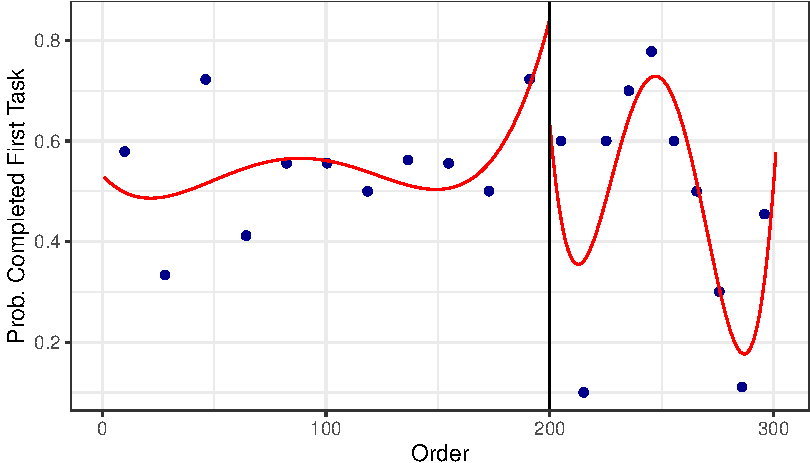
\includegraphics{The-Sources-of-Researcher-Variation-in-Economics_files/figure-pdf/fig-rdd-1.pdf}

}

\caption{\label{fig-rdd}Impact of Guaranteed Payment on Probability of
Task 1 Completion}

\end{figure}

Figure~\ref{fig-rdd} shows no meaningful effect of being guaranteed
payment on the probability of completing Task 1. In additional results
in the appendix, using a linear regression specification of the
regression discontinuity design and the full range of the data (not
including the late sign-ups) to maximize statistical power,\footnote{Use
  of the full range, rather than a bandwidth, is justified given that
  the running variable is randomly assigned aside from the late
  sign-ups. We also find no effect if we drop the late sign-ups from the
  regression discontinuity analysis.} we again find no statistically
significant effect of being guaranteed treatment. This is suggestive
that participants were not simply signing up in an attempt to get a
\$2,000 payment for little effort.

\hypertarget{sec-sample-characteristics}{%
\subsubsection{Sample
Characteristics}\label{sec-sample-characteristics}}

Tables \ref{tab-samp1} to \ref{tab-samp3} show the characteristics of
the recruited sample, and how those characteristics changed with
eligibility and attrition. Task 2 is omitted as an attrition stage since
so few people dropped out between Task 1 and Task 2.

Table \ref{tab-samp1} shows that the majority of researchers were
recruited via social media, with only about 9\% coming from a department
email, 4\% from a professional organization email, and 9\% from some
other source (like word-of-mouth). Those recruited from another source
were less likely to qualify for the study, and slightly less likely to
finish, while those recruited from social media were most likely to
qualify and finish. We also asked researchers how certain they were of
their ability to finish the first task as well as the full set of tasks,
on a scale of 1 to 100. Enrollees were about 90\% confident in their
ability to complete the full set of research tasks (although only about
50\% did). Those who were more confident were slightly more likely to
actually finish, and average confidence rates of those who did finish
were about 92\% instead of 90\%.

\begin{table}[!htbp] \centering \renewcommand*{\arraystretch}{1.1}\caption{Researcher Recruitment Source and Completion Confidence}\label{tab-samp1}\resizebox{\textwidth}{!}{
\begin{tabular}{lrrrrrrrrrrrr}
\hline
\hline
Round & \multicolumn{3}{c}{Original signup} & \multicolumn{3}{c}{Assigned task 1} & \multicolumn{3}{c}{Finished task 1} & \multicolumn{3}{c}{Finished task 3}  \\ 
 Variable & \multicolumn{1}{c}{N} & \multicolumn{1}{c}{Mean} & \multicolumn{1}{c}{SD} & \multicolumn{1}{c}{N} & \multicolumn{1}{c}{Mean} & \multicolumn{1}{c}{SD} & \multicolumn{1}{c}{N} & \multicolumn{1}{c}{Mean} & \multicolumn{1}{c}{SD} & \multicolumn{1}{c}{N} & \multicolumn{1}{c}{Mean} & \multicolumn{1}{c}{SD} \\ 
\hline
Recruitment Source & 347 &  &  & 285 &  &  & 150 &  &  & 142 &  &  \\ 
... Social media & 270 & 78\% &  & 224 & 79\% &  & 124 & 83\% &  & 116 & 82\% &  \\ 
... Department email & 31 & 9\% &  & 28 & 10\% &  & 13 & 9\% &  & 13 & 9\% &  \\ 
... Email of a professional organization & 15 & 4\% &  & 10 & 4\% &  & 4 & 3\% &  & 4 & 3\% &  \\ 
... Other & 31 & 9\% &  & 23 & 8\% &  & 9 & 6\% &  & 9 & 6\% &  \\ 
Certainty to Finish Task 1 & 355 & 90 & 11 & 292 & 90 & 10 & 153 & 92 & 8.4 & 145 & 92 & 8.3 \\ 
Certainty to Finish Task 3 & 355 & 89 & 12 & 292 & 89 & 12 & 153 & 91 & 9.9 & 145 & 91 & 9.6\\ 
\hline
\hline
\end{tabular}
}
\end{table}

Table \ref{tab-samp1} shows the professional experience of enrollees.
While graduate students were considered eligible for the project as long
as they had a published or forthcoming paper, the majority of eligible
researchers (83\%) had PhDs. PhD holders were also more likely than
other eligible researchers to complete all three tasks.

These PhDs are split across faculty (62\%) and other non-faculty
researchers (22\%), both of which were more likely than graduate
students to finish all three rounds. Note that the researchers in these
categories who do not hold PhDs were either people who had been hired to
faculty roles without holding PhDs (such as ABDs, or people in a faculty
position requiring only a Master's degree), or people with Master's
degrees in non-faculty research positions who had published academic
papers (some of whom were still graduate students).

Most of the researchers had at least one published paper, and
researchers with 6+ papers were more likely than others to complete all
three research tasks. Those with ``No Academic Papers'' are non-academic
researchers who produce work not intended for academic journal
publication. Those with ``No Published Academic Papers'' have papers
that are forthcoming, or are faculty who only have working papers and no
publications.

The set of researchers in the study generally do not work in the
specific subfield that the research task is in. The research task is
similar to many studies done across all of applied microeconomics, but
specifically is on the topics of labor and immigration. About a third of
the enrollees had done research in either immigration or labor
previously, and these researchers were somewhat more likely to complete
all three tasks. No researchers enrolled who had previously worked in
both immigration and labor.

\begin{table}[!htbp] \centering \renewcommand*{\arraystretch}{1.1}\caption{Researcher Professional Experience}\label{tab-samp2}\resizebox{\textwidth}{!}{
\begin{tabular}{lrrrrrrrr}
\hline
\hline
Round & \multicolumn{2}{c}{Original signup} & \multicolumn{2}{c}{Assigned task 1} & \multicolumn{2}{c}{Finished task 1} & \multicolumn{2}{c}{Finished task 3}  \\ 
 Variable & \multicolumn{1}{c}{N} & \multicolumn{1}{c}{Percent} & \multicolumn{1}{c}{N} & \multicolumn{1}{c}{Percent} & \multicolumn{1}{c}{N} & \multicolumn{1}{c}{Percent} & \multicolumn{1}{c}{N} & \multicolumn{1}{c}{Percent} \\ 
\hline
Degree & 360 &  & 295 &  & 154 &  & 146 &  \\ 
... No graduate school & 3 & 1\% & 0 & 0\% & 0 & 0\% & 0 & 0\% \\ 
... Some Grad School & 14 & 4\% & 5 & 2\% & 3 & 2\% & 2 & 1\% \\ 
... Master's degree & 78 & 22\% & 44 & 15\% & 17 & 11\% & 17 & 12\% \\ 
... Prof. Degree & 3 & 1\% & 1 & 0\% & 0 & 0\% & 0 & 0\% \\ 
... PhD & 262 & 73\% & 245 & 83\% & 134 & 87\% & 127 & 87\% \\ 
Occupation & 361 &  & 295 &  & 154 &  & 146 &  \\ 
... Faculty & 191 & 53\% & 182 & 62\% & 99 & 64\% & 98 & 67\% \\ 
... Grad. Student & 69 & 19\% & 36 & 12\% & 13 & 8\% & 12 & 8\% \\ 
... Other & 14 & 4\% & 11 & 4\% & 5 & 3\% & 3 & 2\% \\ 
... Other Researcher & 87 & 24\% & 66 & 22\% & 37 & 24\% & 33 & 23\% \\ 
Research Experience & 361 &  & 295 &  & 154 &  & 146 &  \\ 
... 1-5 Papers in Applied Micro & 162 & 45\% & 152 & 52\% & 74 & 48\% & 70 & 48\% \\ 
... 6+ Papers & 104 & 29\% & 102 & 35\% & 58 & 38\% & 57 & 39\% \\ 
... No Academic Papers & 17 & 5\% & 4 & 1\% & 3 & 2\% & 3 & 2\% \\ 
... No Published Academic Papers & 78 & 22\% & 37 & 13\% & 19 & 12\% & 16 & 11\% \\ 
Field & 333 &  & 270 &  & 145 &  & 138 &  \\ 
... Immigration \& Labor & 0 & 0\% & 0 & 0\% & 0 & 0\% & 0 & 0\% \\ 
... Immigration & 8 & 2\% & 6 & 2\% & 4 & 3\% & 4 & 3\% \\ 
... Labor & 102 & 31\% & 85 & 31\% & 49 & 34\% & 47 & 34\% \\ 
... Neither & 223 & 67\% & 179 & 66\% & 92 & 63\% & 87 & 63\%\\ 
\hline
\hline
\end{tabular}
}
\end{table}

While the research tools used are not listed in Table \ref{tab-samp2},
we did check the programming languages used by researchers. The most
common language was Stata, with 109 researchers performing their work
solely in Stata. 33 used R, and one researcher used both R and Stata.
Less common were Python and SPSS, with one researcher each.

Table \ref{tab-samp3} shows the demographics of the researcher sample.
The eligible sample was just under 80\% male and more than 55\% white,
and both percentages grew by the conclusion of Task 3, with the white
share growing significantly to 66\%. The 80\% male figure is similar to
the share male found for faculty at a selected set of top economics
departments in 2017 by Lundberg and Stearns (2019), and among all
actively publishing economists in 2019 by Card et al. (2022). A small
share reported being LGBTQ+, and this share remained constant over all
rounds of the research tasks. An additional form of demographic
difference is geographic. About half of the sample was situated in the
United States, and about half was from another country.\footnote{Exact
  figures are not given for geography, and crosstabulations across
  geography are not given, because non-geographic demographic
  information comes from a survey where we acquired permission to share
  aggregate figures. Geographic information, on the other hand, comes
  from researcher payments information, for which we did not request
  permission to share responses.} The representativeness of the racial
mixture is difficult to assess for this reason; 66\% white would be low
if the entire sample were from the United States (Stansbury and Schultz
2023), but it is unclear what the population rate is in a 50\% US/50\%
other location sample.

\begin{table}[!htbp] \centering \renewcommand*{\arraystretch}{1.1}\caption{Researcher Demographics}\label{tab-samp3}\resizebox{\textwidth}{!}{
\begin{tabular}{lrrrrrrrr}
\hline
\hline
Round & \multicolumn{2}{c}{Original signup} & \multicolumn{2}{c}{Assigned task 1} & \multicolumn{2}{c}{Finished task 1} & \multicolumn{2}{c}{Finished task 3}  \\ 
 Variable & \multicolumn{1}{c}{N} & \multicolumn{1}{c}{Percent} & \multicolumn{1}{c}{N} & \multicolumn{1}{c}{Percent} & \multicolumn{1}{c}{N} & \multicolumn{1}{c}{Percent} & \multicolumn{1}{c}{N} & \multicolumn{1}{c}{Percent} \\ 
\hline
Gender & 359 &  & 294 &  & 154 &  & 146 &  \\ 
... Female & 81 & 23\% & 64 & 22\% & 28 & 18\% & 26 & 18\% \\ 
... Male & 274 & 76\% & 230 & 78\% & 126 & 82\% & 120 & 82\% \\ 
... Non-binary / third gender & 1 & 0\% & 0 & 0\% & 0 & 0\% & 0 & 0\% \\ 
... Prefer not to say & 3 & 1\% & 0 & 0\% & 0 & 0\% & 0 & 0\% \\ 
Race & 360 &  & 294 &  & 154 &  & 146 &  \\ 
... White & 188 & 52\% & 164 & 56\% & 100 & 65\% & 97 & 66\% \\ 
... Asian & 79 & 22\% & 60 & 20\% & 25 & 16\% & 25 & 17\% \\ 
... Black or African American & 27 & 8\% & 21 & 7\% & 4 & 3\% & 4 & 3\% \\ 
... Hispanic & 25 & 7\% & 19 & 6\% & 10 & 6\% & 9 & 6\% \\ 
... Other or Multiracial & 41 & 11\% & 30 & 10\% & 15 & 10\% & 11 & 8\% \\ 
LGBTQ+ & 360 &  & 294 &  & 154 &  & 146 &  \\ 
... Yes & 18 & 5\% & 14 & 5\% & 7 & 5\% & 7 & 5\% \\ 
... No & 323 & 90\% & 268 & 91\% & 137 & 89\% & 129 & 88\% \\ 
... Prefer not to say & 19 & 5\% & 12 & 4\% & 10 & 6\% & 10 & 7\%\\ 
\hline
\hline
\end{tabular}
}
\end{table}

One researcher did complete all three research tasks, and appears in the
above tables, but their work has been removed from the results that
follow in the rest of the paper, because a misunderstanding of the
instructions meant that their work did not attempt to estimate the
effect of DACA on the probability of employment.

As a whole, the sample largely reflects the group of people who publish
work in applied microeconomics. The sample is skewed towards the United
States, which is partially driven by the emails sent to US economics
departments, the fact that the project was advertised and carried out in
English, and the fact that the project organizers are in the United
States and advertised the project using their own social media. Given
that caveat, the makeup of the sample appears to be fairly similar to
the makeup of the profession itself, although this is difficult to
verify for some demographics.

\hypertarget{results}{%
\section{Results}\label{results}}

This section examines the variation in effects and methods across
researchers and conditions, demonstrating that variation exists and
attempting to explain it.

Importantly, these results are derived from the survey responses that
researchers gave about their findings and the choices made. Project
organizers did not cross-reference survey responses against researcher
code to ensure that their code was accurately reflected in the survey,
except in a small number of cases where the survey response could not be
interpreted. This means that the variation presented here represents the
variation in how researchers would plan to implement the research task
if they were doing it independently, and what a reader would see as the
description of a study in a published version of their work. Any
variation between researchers that occurs as a result of coding error or
a research report that misrepresents what a researcher actually did will
not be reflected here, but could be the subject of a future
investigation.

\hypertarget{sec-variation}{%
\subsection{Variation in Effects and Sample Sizes}\label{sec-variation}}

Figure~\ref{fig-effect-distributions} and Table \ref{tab-effectdist}
show the distribution of estimated effects across all researchers. The
effect distributions are shown in two ways: unweighted and using
inverse-standard-error weights.\footnote{The use of
  inverse-standard-error weights is not preregistered but follows
  meta-analytic standards, reducing the influence of estimates that may
  be outliers due to being estimated with a highly-noisy method, under
  the suggestion of Auspurg and Brüderl (2023). Weights are truncated at
  the 95th percentile (200, or a standard error of .005) so as to avoid
  any single researcher having too much influence on results. Not using
  the truncation leads to more agreement because a few researchers with
  very small standard errors make up a significant share of the weighted
  sample.} Several data points are dropped from the weighted analysis
for researchers who did not report standard errors or reported 0. Other
missing values are researchers who did not repond to a given question.

In Task 1, the mean estimated effect of DACA eligibility on the
probability of working full-time was .053 unweighted or .044 weighted.
In both cases these means are pulled upwards by high top-end estimates
and are above the 75th percentiles. Median estimates were .030
unweighted or .026 weighted. Even in Task 1, with a large amount of
freedom afforded, researchers found a reasonable amount of agreement in
the effect sizes outside of the tails, with the 25th to 75th percentile
ranges of the effect being .014 to .051 unweighted, an inter-quartile
range (IQR) of .037, or 3.7 percentage points in the effect, or .012 to
.043 weighted, an IQR of .031. The use of weights narrows the
distribution of effects: researchers reporting smaller standard errors
also reported estimates that were more similar to each other, which was
also the case in Tasks 2 and 3.

Our preregistration plan details that we planned to give descriptive
characteristics of the results, as we do here, and also implement a
Levene test on whether the variance between researchers declined. We do
not reject at the 95\% level the null of no change in variance from any
stage to any later stage (including a comparison of each task to its
revision stage, and comparing each main task to later main tasks), with
the lowest p-value of 0.197 coming from the comparison of Task 1 to Task
1 Revision.

Task 2 is somewhat odd in that it shows less agreement than Task 1
despite giving researchers less freedom. The IQRs increase to .043
unweighted or .040 weighted. Further, the effect distributions are
somewhat bimodal, especially when weighted. One of these modes appears
to be researchers reporting effect estimates of a similar level to those
in Task 1, and others reporting effect estimates similar to what would
later be found in Task 3.

Moving all the way to Task 3, agreement considerably increases between
researchers. The 25th and 75th percentile effects are .031 and .058
unweighted (IQR .027), and .036 and .060 weighted (IQR .024). The
bimodality from Task 2 is still there, but with much more agreement and
density at the higher mode. From Round 1 to Round 3 we see considerable
increases in agreement between researchers.

Taking only the effect distributions as a baseline, we see that, at
least in this application, researchers in general report fairly similar,
although certainly not identical, effect estimates on average, but there
are some extreme outlier estimates as well. We may also take this to
mean that providing pre-cleaned data, as in Task 3, led to a strong
increase in researcher agreement. Specifying further the research
question and design, however, as in Task 2, led to somewhat less
agreement. The odd result for Task 2 and its proper interpretation will
be investigated further in Section~\ref{sec-bimodal}.

\begin{figure}

{\centering 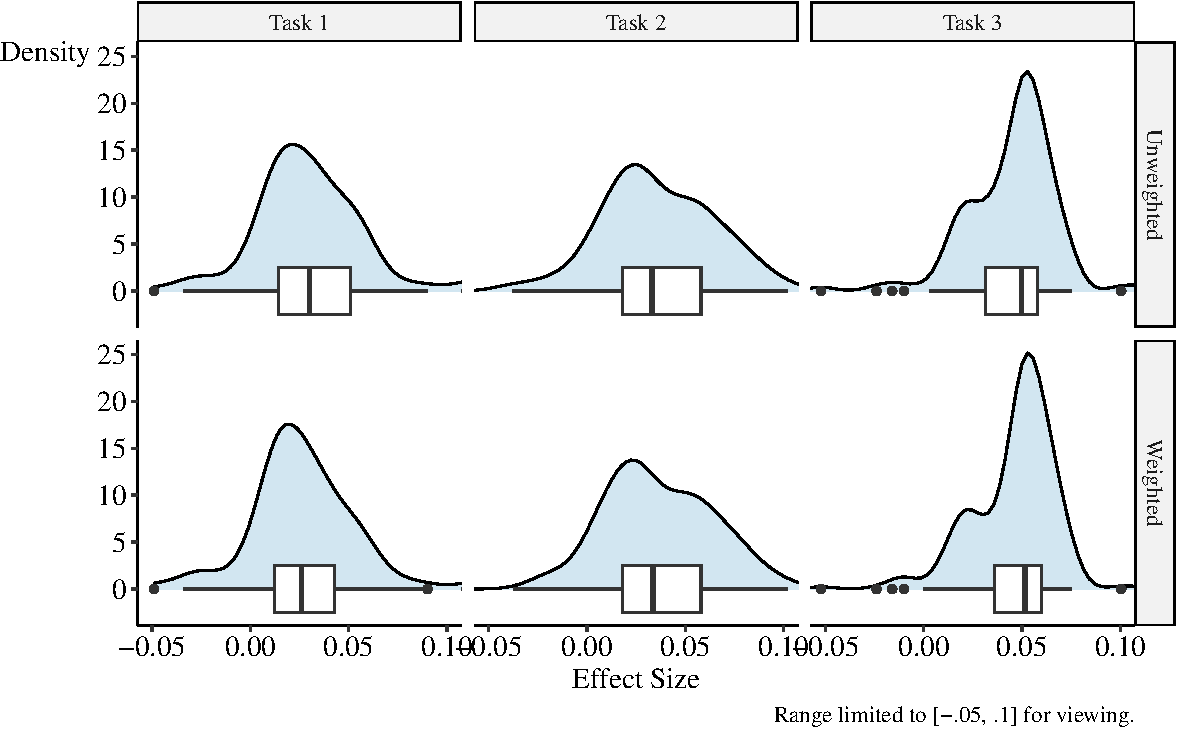
\includegraphics{The-Sources-of-Researcher-Variation-in-Economics_files/figure-pdf/fig-effect-distributions-1.pdf}

}

\caption{\label{fig-effect-distributions}Distributions of Reported
Effect Sizes}

\end{figure}

Table \ref{tab-effectdist} also shows the reported standard errors.
Reported standard errors increase significantly from round to round,
driven largely by the specification of the research design, which for
many researchers considerably narrowed the sample they were supposed to
use. This can also be seen in Figure~\ref{fig-full-effect-distribution},
where the distribution of effects narrows a little across rounds, but
confidence intervals increase considerably. Throughout, while there is
general agreement on effect size in the middle of the distribution,
researchers vary in whether the reported effect is statistically
significant, with 78\%, 60\%, and 64\% reporting results that were
statistically significantly different from 0 in Tasks 1, 2, and 3,
respectively.

We can compare average standard errors against the variation in effects
between researchers to get a sense of how much effect variability is
omitted by only considering a reported standard error, as in
Huntington-Klein et al. (2021) or Menkveld et al. (2021). Comparing the
standard deviation of weighted effects against the average standard
error gives ratios of 4.84, 2.23, and 1.75 for Tasks 1, 2, and 3,
respectively. Huntington-Klein et al. (2021) used a single round and
allowed full researcher freedom, and found a range of 3-4 for this
ratio, below what we find for the full-freedom Task 1. If we instead
compare weighted IQR to average standard errors we get ratios of 1.63,
1.29, and .41. The decrease over rounds is partially driven by
increasing agreement over rounds, which suggest that a reported standard
error considerably understates the estimate uncertainty that we should
acknowledge when including researcher variation. However, these
reductions are also driven by the fact that sample sizes decreased from
round to round, due to the shared research design instructing
researchers to use a more restricted sample than many used in Task 1.
These reduced sample sizes increased the reported standard errors and
thus the denominator of the effect-variation-to-average-standard-error
ratio. This behavior demonstrates a flaw with these ratios, introduced
in Huntington-Klein et al. (2021), as a metric for researcher-indused
uncertainty. Even if one might expect that researcher variation should
be higher for research designs with smaller samples (or less precision
for some other fundamental reason), there's no reason to believe that
researcher variation would scale at the same rate as the standard error.
So this ratio will tend to be higher for research tasks with bigger
samples than smaller samples, even if the level of researcher variation
is the same.

\begin{table}[!htbp] \centering \renewcommand*{\arraystretch}{1.1}\caption{Distribution of Reported Effects and Sample Sizes}\label{tab-effectdist}\resizebox{\textwidth}{!}{
\begin{tabular}{lllllllll}
\hline
\hline
Variable & N & Mean & SD & Min & Pctl. 25 & Median & Pctl. 75 & Max \\ 
\hline
\multicolumn{9}{c}{Round: Task 1} \\ 
Effect Size (Unweighted) & 145 & 0.053 & 0.095 & -0.049 & 0.014 & 0.030 & 0.051 & 0.660 \\ 
Effect Size (Weighted) & 138 & 0.044 & 0.092 & -0.049 & 0.012 & 0.026 & 0.043 & 0.660 \\ 
Standard Error & 139 & 0.019 & 0.055 & 0.000 & 0.005 & 0.007 & 0.013 & 0.460 \\ 
Sample Size & 145 & 828,318 & 3,056,037 & 681 & 61,600 & 179,960 & 356,787 & 29,536,580 \\ 
Treated-Group Size & 141 & 96,395 & 648,493 & 270 & 17,950 & 34,435 & 52,581 & 7,727,201 \\ 
\multicolumn{9}{c}{Round: Task 2} \\ 
Effect Size (Unweighted) & 145 & 0.044 & 0.100 & -0.390 & 0.015 & 0.032 & 0.058 & 0.850 \\ 
Effect Size (Weighted) & 141 & 0.046 & 0.069 & -0.090 & 0.018 & 0.034 & 0.058 & 0.850 \\ 
Standard Error & 141 & 0.031 & 0.078 & 0.001 & 0.010 & 0.014 & 0.020 & 0.744 \\ 
Sample Size & 144 & 157,006 & 1,065,593 & 6,196 & 18,981 & 25,414 & 48,125 & 12,609,847 \\ 
Treated-Group Size & 140 & 31,948 & 221,175 & 3,519 & 5,953 & 11,157 & 15,832 & 2,627,183 \\ 
\multicolumn{9}{c}{Round: Task 3} \\ 
Effect Size (Unweighted) & 145 & 0.045 & 0.101 & -0.810 & 0.031 & 0.050 & 0.058 & 0.650 \\ 
Effect Size (Weighted) & 142 & 0.062 & 0.103 & -0.810 & 0.036 & 0.051 & 0.060 & 0.650 \\ 
Standard Error & 144 & 0.059 & 0.268 & 0.000 & 0.015 & 0.018 & 0.026 & 2.747 \\ 
Sample Size & 145 & 16,904 & 1,756 & 7,833 & 17,379 & 17,382 & 17,382 & 17,832 \\ 
Treated-Group Size & 129 & 9,433 & 3,008 & 11 & 5,149 & 11,382 & 11,382 & 17,383\\ 
\hline
\hline
\end{tabular}
}
\end{table}

\begin{figure}

{\centering 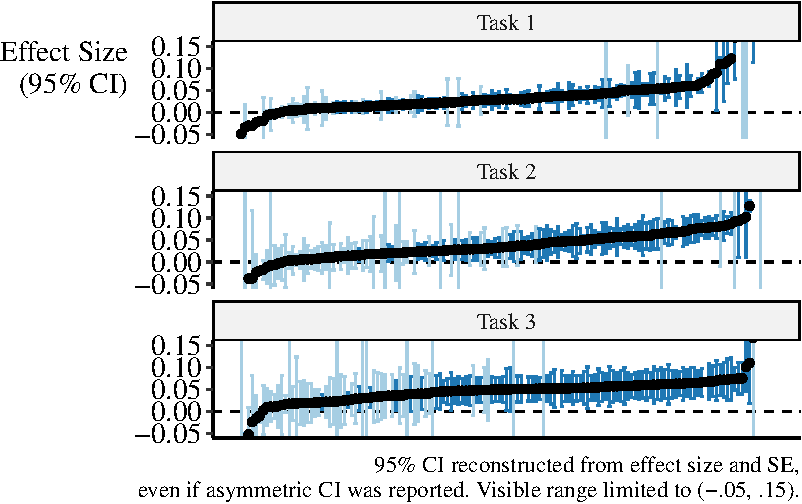
\includegraphics{The-Sources-of-Researcher-Variation-in-Economics_files/figure-pdf/fig-full-effect-distribution-1.pdf}

}

\caption{\label{fig-full-effect-distribution}Specification Curve for All
Reported Estimates}

\end{figure}

Table \ref{tab-effectdist} also shows summary statistics for reported
standard errors, both overall and for the treated group. These
distributions are also shown in
Figure~\ref{fig-sample-size-distributions} and
Figure~\ref{fig-treated-group-distributions}.

In Figure~\ref{fig-sample-size-distributions} we see a huge amount of
variation in the reported sample size used in Task 1, noting that the
x-axis is on a log scale. The 25th and 75th percentiles of reported
sample sizes ranging from 61,600 to 356,787, with some researchers using
millions of observations.\footnote{Keep in mind that for Task 1, there
  was not a specified control group, so a researcher may decide to use
  the entire ACS sample in the analysis, including people very unlike
  the eligible group in the sample. In Task 2, the instructions
  specified a treated and comparison group, but some researchers may
  have different samples than in Task 3 either due to error, or because
  they included people other than the treated and comparison group in
  their sample to improve precision, and used their model to compare
  those groups more directly.} For Task 2, which specified in the
instructions the treated and comparison groups to use, variation reduces
considerably, although the 75th percentile (48,125) is still double the
25th (18,981), and there are still some researchers using millions of
observations. Task 3 is not shown in the graph because the sample is
pre-specified, with the only meaningful variation being whether or not
the researcher dropped three rows of data with missing education values,
and a few outliers reporting lower numbers. The lower sample sizes for
this question are due to researchers who skipped it because they assumed
the answer was obvious.

\begin{figure}

{\centering 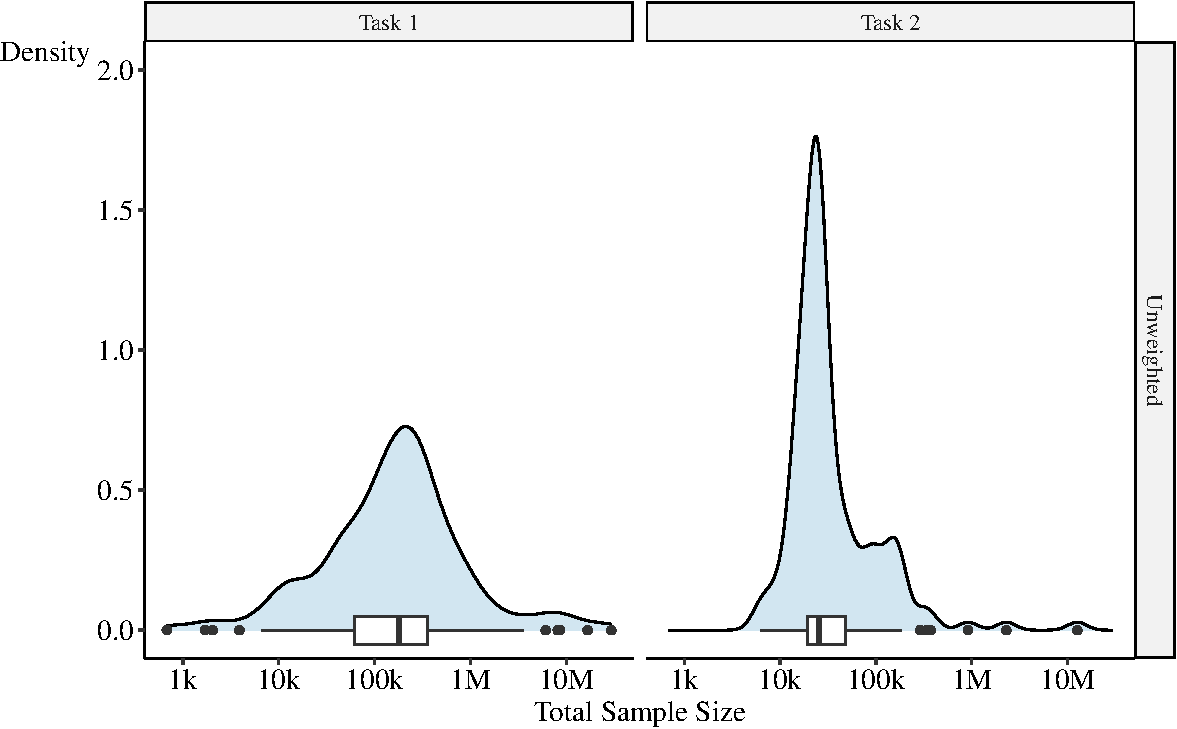
\includegraphics{The-Sources-of-Researcher-Variation-in-Economics_files/figure-pdf/fig-sample-size-distributions-1.pdf}

}

\caption{\label{fig-sample-size-distributions}Distributions of Reported
Sample Sizes}

\end{figure}

Variation in the reported size of the treated group in
Figure~\ref{fig-treated-group-distributions} is affected somewhat by
researcher confusion in responding to the survey question. The survey
question about treated-group size instructed researchers not to count
individuals eligible for DACA as treated for the purposes of this
question if they were in a pre-DACA year. However, many researchers
counted these individuals as treated anyway, leading to variation in the
Task 3 distribution, even though every researcher is at this point
working with the same eligibility indicator.

\begin{figure}

{\centering 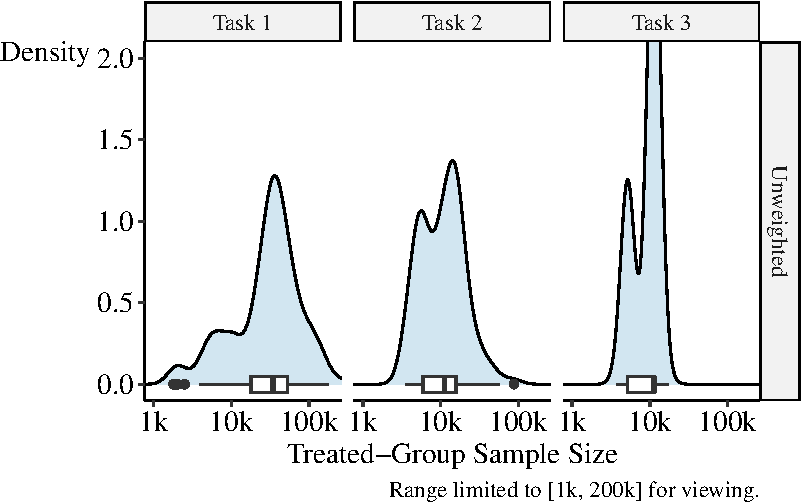
\includegraphics{The-Sources-of-Researcher-Variation-in-Economics_files/figure-pdf/fig-treated-group-distributions-1.pdf}

}

\caption{\label{fig-treated-group-distributions}Distributions of
Reported Treated-Group Sizes}

\end{figure}

Aside from this issue, we see that the imposition of a shared definition
for the trated group reduced the IQR for the size of the group from
34,631 in Taks 1 to 9,879 in Task 2. Theoretically, however, since there
was a shared definition of the treated group in Task 2, there should be
no more variation in this variable in Task 2 than in Task 3. This
indicates that not all instructions were implemented in the same way
across researchers, which will be explored further in
Section~\ref{sec-sample-limitations}. Despite a shared understanding of
who was eligible for DACA and who should be in the treated group, only a
shared data preparation that implemented these rules for people led to
sharp agreement in the size of the treated-groups sample.

\hypertarget{peer-review}{%
\subsection{Peer Review}\label{peer-review}}

This section evaluates the impact of peer review on the later work
performed by a researcher. The structure of peer review in this study is
that, following each main task, 2/3 of the researchers are randomized
into pairs that produce a peer review report of the other's work, while
the remaining 1/3 do not receive or perform peer review. Then,
researchers have an opportunity to revise their work.

Revision is optional, and relatively few researchers (fewer than 30 per
task) chose to revise their work after receiving peer review. As such,
we mostly look at the impact of peer review on the work performed in
subsequent main tasks. However, we can check if revision tended to lead
towards more agreement overall. In Table
\ref{tab-variance-after-revision}, we show the variance of the entire
sample of reported effects post-revision, replacing each researcher's
reported task effect with its revision, if they revised their work, and
compare variance among the peer-reviewed group to the non-peer-reviewed
group. At no point is this difference statistically significant, and it
is inconsistent which group had the lower post-revision variance. Taking
only the subgroup of actually-revised estimates, we see that these
tended to agree with each other more than the group as a whole did in
Tasks 1 and 2, but this is also inconsistent, with greater variance than
the whole group in Task 3 and when pooling over all tasks (after
subtracting by-task means).

\begin{longtable}[]{@{}
  >{\raggedright\arraybackslash}p{(\columnwidth - 8\tabcolsep) * \real{0.0854}}
  >{\raggedright\arraybackslash}p{(\columnwidth - 8\tabcolsep) * \real{0.2439}}
  >{\raggedright\arraybackslash}p{(\columnwidth - 8\tabcolsep) * \real{0.2195}}
  >{\raggedright\arraybackslash}p{(\columnwidth - 8\tabcolsep) * \real{0.2439}}
  >{\raggedright\arraybackslash}p{(\columnwidth - 8\tabcolsep) * \real{0.2073}}@{}}
\caption{Post-Revision Variance by Peer Review
\label{tab-variance-after-revision}}\tabularnewline
\toprule\noalign{}
\begin{minipage}[b]{\linewidth}\raggedright
Task
\end{minipage} & \begin{minipage}[b]{\linewidth}\raggedright
Unreviewed Variance
\end{minipage} & \begin{minipage}[b]{\linewidth}\raggedright
Reviewed Variance
\end{minipage} & \begin{minipage}[b]{\linewidth}\raggedright
Levene Test p-value
\end{minipage} & \begin{minipage}[b]{\linewidth}\raggedright
Revised Variance
\end{minipage} \\
\midrule\noalign{}
\endfirsthead
\toprule\noalign{}
\begin{minipage}[b]{\linewidth}\raggedright
Task
\end{minipage} & \begin{minipage}[b]{\linewidth}\raggedright
Unreviewed Variance
\end{minipage} & \begin{minipage}[b]{\linewidth}\raggedright
Reviewed Variance
\end{minipage} & \begin{minipage}[b]{\linewidth}\raggedright
Levene Test p-value
\end{minipage} & \begin{minipage}[b]{\linewidth}\raggedright
Revised Variance
\end{minipage} \\
\midrule\noalign{}
\endhead
\bottomrule\noalign{}
\endlastfoot
Task 1 & 0.002 & 0.012 & 0.173 & 0.001 \\
Task 2 & 0.009 & 0.004 & 0.571 & 0.002 \\
Task 3 & 0.001 & 0.008 & 0.210 & 0.015 \\
Pooled & 0.004 & 0.008 & 0.219 & 0.005 \\
\end{longtable}

In general, the mechanisms by which peer review might be expected to
change a researcher's work in normal journal submissions include both
that researchers might find peer review comments helpful and incorporate
them into their work, and that researchers are required by the journal
submission process to incorporate most reviewer comments. In this study,
our peer review process can only capture the first of these mechanisms,
and in effect may be closer to comments received, for example, during
seminar presentations.

Figure~\ref{fig-peer-review-effect-distributions} shows the distribution
of effect sizes estimated by those who did, and did not, engage in peer
review in each round. The left column of graphs shows the effects
reported in each task before researchers were assigned to peer review,
and the right column shows the effects reported in the follow-up task,
comparing those either assigned or not assigned to peer review in the
previous task. As we might expect given random assignment, effect
distributions are fairly similar pre-review between the review and
non-review groups, with a slightly narrower distribution of effects for
researchers about to be reviewed.

We also see that these groups have very similar effect distributions in
their follow-up task. Neither group has a considerably narrower
distribution than the other. Levene tests for differences in follow-up
round effect variance between the peer-reviewed and non-peer-reviewed
groups show p-values of 0.846 and 0.788 in Tasks 2 and 3, respectively,
or 0.999 when pooling the two tasks. This is not strong evidence in
favor of the idea that peer review might drive agreement between
researchers due to the receipt of feedback.

\begin{figure}

{\centering 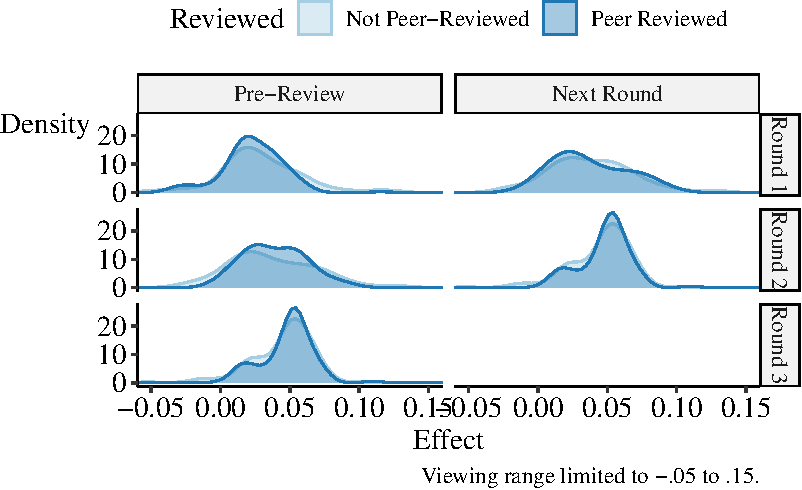
\includegraphics{The-Sources-of-Researcher-Variation-in-Economics_files/figure-pdf/fig-peer-review-effect-distributions-1.pdf}

}

\caption{\label{fig-peer-review-effect-distributions}Distributions of
Reported Effect Sizes}

\end{figure}

Figure~\ref{fig-like-your-reviewer} explores the possibility that peer
review might not make the peer-reviewed group as a whole more similar,
but rather just make someone more similar to their specific reviewer. We
calculate the absolute difference in effects between each reviewer pair,
in the task they perform before reviewing (left column), in the
follow-up task (middle column) and comparing your follow-up task against
your reviewer's result this round (right column), with the right column
representing the possibility that a researcher may select an analysis so
as to produce a result more similar to the one they saw in the previous
round. The distributions of absolute differences for non-reviewed
researchers are generated as a null distribution by matching every
non-reviewed researcher to every other non-reviewed researcher and
calculating all absolute differences.\footnote{This null distribution
  represents the distribution of absolute differences among people who
  did not actually experience peer review. Notably, each non-reviewer is
  matched multiple times in this approach, instead of just once for
  reviewers. However, matching the non-reviewers only once to a single
  random pair just produces a noisier version of this all-matches null
  distribution. Averaging the single-random-match approach over many
  random single matches produces the same null distribution.}

In Figure~\ref{fig-like-your-reviewer} we see some of the anticipated
effect of peer review for Task 1. Before review (left column), absolute
differences between review pairs were more likely to be large than
differences between non-review pairs. But by the follow-up in Task 2,
both groups were similar, potentially suggesting that peer review
reduced the large absolute differences. In the right column, the
unreviewed group still shows lower differences, but to a smaller degree.
However, none of this holds up in Task 2. Again the actual review pairs
started out with larger differences, and those differences shrank for
both groups by Task 3, but by the same degree. Appendix Table
\ref{tab-peer-review-reg} shows that average absolute differences grew
by a statistically significant .051 more for the unreviewed group than
for the reviewed group in Task 1, but that this effect reverses to a
statistically significant .029 in favor of the unreviewed group for Task
2. This is not consistent strong evidence of peer review making a
researcher more like their reviewer as the result of feedback.

\begin{figure}

{\centering 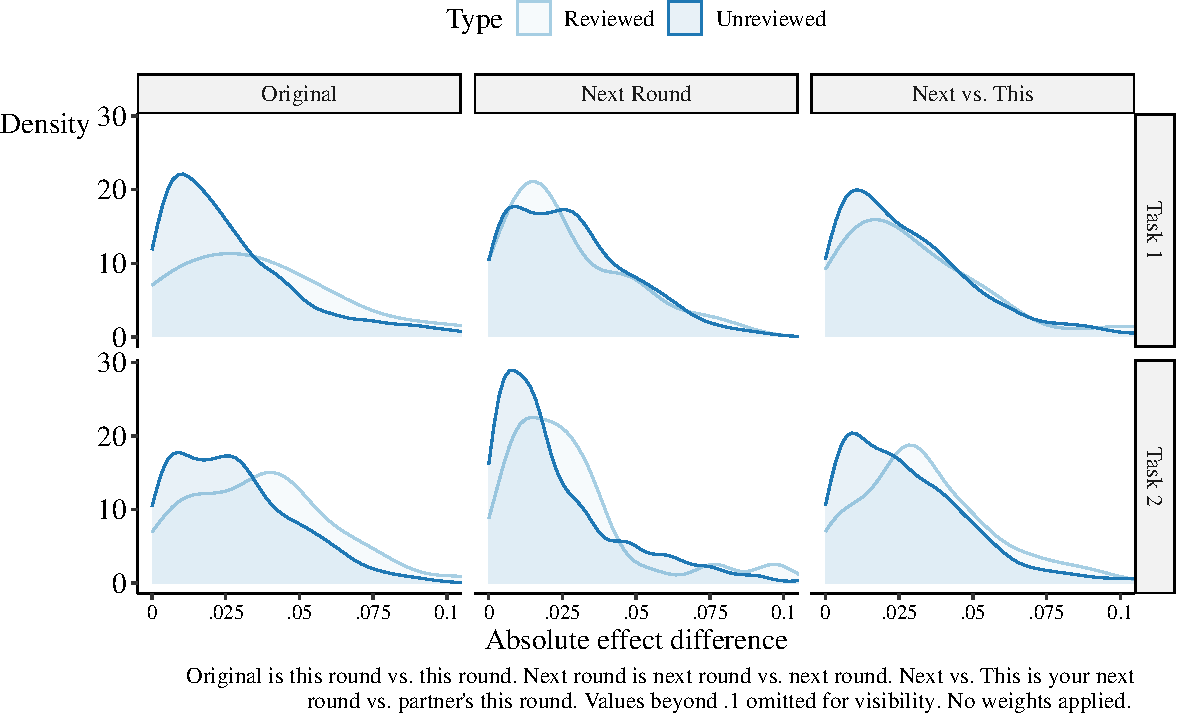
\includegraphics{The-Sources-of-Researcher-Variation-in-Economics_files/figure-pdf/fig-like-your-reviewer-1.pdf}

}

\caption{\label{fig-like-your-reviewer}Comparisons of Effect Sizes
vs.~One's Reviewer}

\end{figure}

\hypertarget{sec-analytic}{%
\subsection{Analytic Choices}\label{sec-analytic}}

The next two sections examine the different choices that researchers
made, both to demonstrate the variation in ways that different
researchers chose to carry out the research tasks, and to relate those
choices to differences in outcomes.

Table \ref{tab-estimation-methods} shows the different choices made in
estimating the effect of DACA on the probability of employment across
all three tasks, in particular the estimator chosen, the use of ACS
sampling weights provided by IPUMS, and the choice of standard error
adjustment.\footnote{For most researchers, these choices did not change
  over the tasks, and so we just present the overall view.} The
dependent variable of interest, working full-time or not, is binary.
However, as is generally standard in applied microeconomics, linear
regression was the most common estimator used, with 82\% of entries.
13\% used logit or probit regression instead. Notably, many reserachers
used linear regression as a means of implementing a fully saturated (or
nearly fully saturated) difference-in-differences design, in which case
the downsides of linear probability models are muted. Other researchers
mostly used a matching estimator (sometimes combined with linear
regression) or one of several newly-introduced estimators for
difference-in-differences designs, like Callaway and Sant'Anna (2021).

The use of sample weights was relatively uncommon, despite their use
being advised with survey data like ACS. Only 25\% of task completions
mentioned the use of weights or any of the standard ACS weight
variables.

There was considerable variation across researchers in the selection of
standard error adjustment. A slim majority of researchers applied
clustered standard errors in some way, but clustered at different
levels: state, state/year, or according to a survey clustering indicator
like Strata or some other variable. A further 17\% of submissions used
heteroskedasticity-robust but not cluster-robust standard errors.

\begin{table}[!htbp] \centering \renewcommand*{\arraystretch}{1.1}\caption{Estimation Methods}\label{tab-estimation-methods}\resizebox{\textwidth}{!}{
\begin{tabular}{lrr@{\hskip .1in}lrr}
\hline
\hline
Variable & N & Percent & Variable & N & Percent \\ 
\hline
Method & 437 &  & S.E. Adjustment & 438 &  \\ 
... Linear Regression & 358 & 82\% & ... Cluster (State) & 118 & 27\% \\ 
... Logit/Probit & 57 & 13\% & ... Cluster (State \& Year) & 58 & 13\% \\ 
... Matching & 11 & 3\% & ... Cluster (ID/Strata/Other) & 65 & 15\% \\ 
... New DID Estimator & 7 & 2\% & ... Het-Robust & 76 & 17\% \\ 
... Other & 4 & 1\% & ... Other/Bootstrap & 23 & 5\% \\ 
Weights & 438 &  & ... None & 98 & 22\% \\ 
... No Sample Weights & 329 & 75\% &  &  &  \\ 
... Sample Weights & 109 & 25\% &  &  & \\ 
\hline
\hline
\multicolumn{6}{l}{\begin{tabular}[x]{@{}r@{}}This table shows details on estimation, not research design. "Difference-in-differences" \\ implemented with linear regression, for example, counts here as linear regression.\end{tabular}}\\ 
\end{tabular}
}
\end{table}

Table \ref{tab-controls-across-rounds} shows the average rate of
inclusion of covariates across all three tasks. These can be read as the
share of researchers who included the covariate, with the exception of
``Other'', which allows each researcher to have multiple ``Other''
controls. The most common covariates included are shown, with the
exception of indicators for ``eligible for DACA'' or ``in a post-DACA
period'', as these are considered part of the core research design
rather than covariates. Variables are included here regardless of the
functional form used to include them.

The most common included controls were for state, year, age, and sex,
which were included as covariates for more than 50\% of researchers in
all three tasks. However, there was heavy variation in the sets of
included covariates. In Task 1, for example, there are ten covariates
with rates between .2 and .8, meaning that at least 20\% of the
researchers made a different decision on inclusion of the covariate than
the majority. There are four covariates in the 40-60\% range, meaning
that the researchers were almost evenly split on whether or not to
include the covariate. These rates did not change much by Task 3.

Across all rounds, in which there were 435 submitted research tasks,
there were 333 different unique sets of included covariates after
``Other'' covariates are excluded. 64\% of submissions had a set of
covariates that was unique for the task. 17\% shared a covariate set
with one other person in that task, 12\% shared with two or three other
people, and only the those with no controls shared with more than three
other people.

\begin{longtable}[]{@{}llll@{}}
\caption{Average Rate of Covariate Inclusion Across Rounds
\label{tab-controls-across-rounds}}\tabularnewline
\toprule\noalign{}
Control & Task 1 & Task 2 & Task 3 \\
\midrule\noalign{}
\endfirsthead
\toprule\noalign{}
Control & Task 1 & Task 2 & Task 3 \\
\midrule\noalign{}
\endhead
\bottomrule\noalign{}
\endlastfoot
Age & 0.62 & 0.57 & 0.52 \\
Age at Migration & 0.18 & 0.14 & 0.14 \\
Age in 2012 & 0.05 & 0.04 & 0.08 \\
Continuous Years in USA & 0.13 & 0.13 & 0.12 \\
Education & 0.48 & 0.50 & 0.51 \\
English Speaker & 0.17 & 0.17 & 0.23 \\
Labor Force Participation Rate & 0.22 & 0.17 & 0.20 \\
Marital Status & 0.10 & 0.13 & 0.12 \\
Race & 0.24 & 0.22 & 0.28 \\
Sex & 0.63 & 0.64 & 0.72 \\
State & 0.62 & 0.64 & 0.64 \\
State Policy Variables & 0.25 & 0.21 & 0.23 \\
Unemployment Rate & 0.32 & 0.27 & 0.30 \\
Year & 0.68 & 0.60 & 0.57 \\
Year of Migration & 0.14 & 0.13 & 0.11 \\
Other & 0.66 & 0.63 & 0.63 \\
None & 0.07 & 0.07 & 0.06 \\
\end{longtable}

There was very little agreement across researchers on the exact set of
appropriate controls, or the inclusion or exclusion of any given control
(aside from those very rarely included). Did these choices impact the
effect estimates? Not by much. Table \ref{tab-effects-by-controls} shows
the average effect among researchers who included a given control,
pooling all three tasks. The mean reported effects differ by only .023
percentage points comparing the covariate included in analyses with the
highest average effectestimates (Continuous Years in the USA) against
the lowest (Race). This likely overstates the impact of covariate
selection here, as selecting the highest vs.~lowest after estimates are
known will bias us towards a larger difference from noise alone.

There do not appear to be major differences in the average reported
standard errors either, or in the standard deviation of the effect
distribution among reserachers including that covariate.

\begin{longtable}[]{@{}lrlll@{}}
\caption{Estimated Effects by Control-Variable Inclusion
\label{tab-effects-by-controls}}\tabularnewline
\toprule\noalign{}
Control & N & Effect & Mean SE & Effect SD \\
\midrule\noalign{}
\endfirsthead
\toprule\noalign{}
Control & N & Effect & Mean SE & Effect SD \\
\midrule\noalign{}
\endhead
\bottomrule\noalign{}
\endlastfoot
Continuous Years in USA & 55 & 0.054 & 0.035 & 0.123 \\
Age & 248 & 0.048 & 0.025 & 0.094 \\
Year of Migration & 55 & 0.048 & 0.033 & 0.112 \\
Marital Status & 51 & 0.047 & 0.016 & 0.071 \\
Sex & 289 & 0.046 & 0.027 & 0.101 \\
Age at Migration & 67 & 0.045 & 0.022 & 0.067 \\
None & 28 & 0.045 & 0.060 & 0.133 \\
State & 275 & 0.045 & 0.025 & 0.089 \\
Year & 267 & 0.045 & 0.026 & 0.094 \\
Education & 216 & 0.042 & 0.017 & 0.061 \\
Other & 278 & 0.040 & 0.038 & 0.086 \\
Age in 2012 & 24 & 0.037 & 0.026 & 0.042 \\
State Policy Variables & 99 & 0.037 & 0.033 & 0.108 \\
Unemployment Rate & 128 & 0.036 & 0.033 & 0.097 \\
Labor Force Participation Rate & 86 & 0.035 & 0.041 & 0.115 \\
English Speaker & 82 & 0.034 & 0.046 & 0.100 \\
Race & 106 & 0.031 & 0.032 & 0.092 \\
\end{longtable}

While the inclusion of a given common control variable does not strongly
predict an estimated effect, in Table
\ref{tab-effects-by-functional-form} we look at the most common
covariates and examine whether their functional form meaningfully
affects the estimated effect. The selection of functional form explained
more variation in average estimated effects than the inclusion of
covariates did, at least in this context. For both age and the
State/Year controls, the difference between the highest-average-effect
functional form variants and the lowest, in both cases comparing a
linear control against a fixed effect, was greater than the difference
between highest and lowest among covariates included.

\begin{longtable}[]{@{}llrlll@{}}
\caption{Estimated Effects by Functional Form of Control Variable
\label{tab-effects-by-functional-form}}\tabularnewline
\toprule\noalign{}
Category & Control & N & Effect & Mean SE & Effect SD \\
\midrule\noalign{}
\endfirsthead
\toprule\noalign{}
Category & Control & N & Effect & Mean SE & Effect SD \\
\midrule\noalign{}
\endhead
\bottomrule\noalign{}
\endlastfoot
AGE & Linear Age & 164 & 0.058 & 0.024 & 0.107 \\
AGE & Age FE & 36 & 0.024 & 0.040 & 0.022 \\
AGE & Age Quadratic & 33 & 0.035 & 0.015 & 0.089 \\
EDUC & Linear Education & 122 & 0.040 & 0.016 & 0.066 \\
EDUC & Education FE & 32 & 0.047 & 0.021 & 0.033 \\
EDUC & Education Transform & 61 & 0.045 & 0.017 & 0.064 \\
STATE/YEAR & Linear Year & 79 & 0.044 & 0.037 & 0.140 \\
STATE/YEAR & Year FE & 103 & 0.047 & 0.026 & 0.062 \\
STATE/YEAR & State FE & 155 & 0.046 & 0.031 & 0.102 \\
STATE/YEAR & State FE x Year FE & 56 & 0.037 & 0.018 & 0.027 \\
STATE/YEAR & State FE x Linear Year & 23 & 0.061 & 0.017 & 0.133 \\
\end{longtable}

These specific findings about the impact of choices on effects - that
the inclusion of different covariates did not have a major impact on
estimated effects, or that the choice of functional form had a greater
impact than the selection of covariates - should not be expected to
generalize, and is specific to this research task. However, what we can
take from this section is that there is substantial variation across
researchers in what they believe the appropriate set of covariates to be
and, for a given covariate, what the appropriate functional form is. We
can also see that, in the case of this particular study, these
decisions, while varied, did not fully explain the variation in effects
between researchers.

\hypertarget{sec-sample-limitations}{%
\subsection{Sample Limitations}\label{sec-sample-limitations}}

In this section we examine the ways in which researchers defined their
analytic samples, as well as defined the treated group, and any
comparison group included in the data analysis that was not treated.
These data are derived from researcher responses to a survey about their
work, in which they were asked to describe how they limited the size of
their sample before downloading it from IPUMS and which variables they
used to further drop observations from the sample before analysis. For
example someone might say that they only kept observations for which
HISPAN == 1 (the observation is Hispanic-Mexican), along with other
restrictions. These two responses are combined to define the full
analytic sample.

Researchers were also asked to describe how they defined the treated
group who was affected by DACA. For example someone might say that only
those with CITIZEN == 3 (non-citizens) were eligible, along with other
restrictions. These were combined with the analytic-sample restrictions
to make the full treated group definition. Finally, researchers were
similarly asked to describe the conditions that defined someone who
would be included in analysis but not be treated by DACA, which were
combined with the analytic-sample restructions to make the full
comparison group definition.

Researchers were asked to specify these conditions as precisely as
possible to match what they did, and to use IPUMS variable names in
their descriptions. The project organizers coded these into a set of
boolean conditions defining the overall sample, treated group, and
comparison group for each researcher, in some cases reviewing the code
directly or asking researchers to clear up uncertainty where survey
responses were unclear, but in general taking the researcher survey
responses at their word. For these analyses, Task 3 is omitted because
the analytic sample is defined for all researchers.

Table \ref{tab-number-of-sample-limitations} looks purely at the number
of distinct variables referenced in the sample limitations, regardless
of what they are. In Task 1, the typical researcher used five variables
to define their analytic sample, and an additional four to define their
treated group. In Task 2, where inclusion criteria were shared, both of
these numbers increased, but there was still considerable variation,
with the 25th and 75th percentiles using 3 and 10 variables to define
their full sample. Definition of the treated group was more shared, with
the 25th and 75th percentiles using 9 and 12 variables, respectively.

\begin{table}[!htbp] \centering \renewcommand*{\arraystretch}{1.1}\caption{Number of Variables Referred to in Sample Limitations}\label{tab-number-of-sample-limitations}\resizebox{\textwidth}{!}{
\begin{tabular}{lrrrrrrrr}
\hline
\hline
Variable & \multicolumn{1}{c}{N} & \multicolumn{1}{c}{Mean} & \multicolumn{1}{c}{Std. Dev.} & \multicolumn{1}{c}{Min} & \multicolumn{1}{c}{Pctl. 25} & \multicolumn{1}{c}{Pctl. 50} & \multicolumn{1}{c}{Pctl. 75} & \multicolumn{1}{c}{Max} \\ 
\hline
\multicolumn{9}{c}{Round: Task 1} \\ 
Whole Sample & 145 & 5.0 & 2.7 & 0.0 & 3.0 & 5.0 & 7.0 & 14.0 \\ 
Treated Group & 145 & 8.6 & 2.1 & 3.0 & 7.0 & 9.0 & 10.0 & 17.0 \\ 
Untreated Group & 145 & 8.0 & 2.7 & 1.0 & 7.0 & 8.0 & 10.0 & 17.0 \\ 
 &  &  &  &  &  &  &  &  \\ 
\multicolumn{9}{c}{Round: Task 2} \\ 
Whole Sample & 145 & 6.8 & 3.9 & 0.0 & 3.0 & 8.0 & 10.0 & 15.0 \\ 
Treated Group & 145 & 10.3 & 2.3 & 3.0 & 9.0 & 10.0 & 12.0 & 16.0 \\ 
Untreated Group & 145 & 10.2 & 2.3 & 3.0 & 9.0 & 10.0 & 12.0 & 16.0\\ 
\hline
\hline
\end{tabular}
}
\end{table}

As for how those variables are actually used, Table
\ref{tab-sample-limitations-extensive} shows how these variables were
implemented as sample restrictions. Importantly, these reflect the
survey responses given by researchers. Some of the ``none'' responses in
Task 2 in particular reflect researchers who did use the variable in
some way but did not report it in their description of
results.\footnote{Other notes of interest for reading the table: (a)
  ``Multistep condition'' refers to cases where the variable is
  included, but only as a part of a complex boolean statement involving
  many variables. These most commonly appeared in definitions for the
  comparison group, which are not in the table, in the format of ``fails
  any one of the following set of DACA eligibility requirements.'' and
  (b) for Education/Veteran status, recall that the mention of this
  eligibility requirement was omitted from the Task 1 instructions,
  which explains why very few researchers used these variables to define
  their samples or treated groups in Task 1.}

We see a huge amount of variety in the ways these variables were used,
including in Task 2 for the treated-group definition, where there is a
correct answer according to the instructions (and similarly a correct
answer for some variables in the Task 1 treated-group
definition).\footnote{Keep in mind also that these are recoded versions
  of the actual survey submissions sent in by researchers. The survey
  question asked respondents to use IPUMS variable names to describe
  their choices. So for example the individuals reporting that they used
  only high school graduates or \emph{non-veterans,} instead of veterans
  as per the instructions, likely did not intentionally choose to use
  non-veterans and write ``I chose to use non-veterans in my sample'' in
  their response but rather they wrote ``VETSTAT == 1,'' which indicates
  ``non-veteran'', perhaps based on a misunderstanding of the IPUMS
  documentation (veterans are VETSTAT == 2).} For each variable, the
most-common option, listed at the top, is the ``correct'' answer for
defining the treated group, with two exceptions: (a) for Citizenship,
there is a second justifiable answer in ``Non-Citizen or Naturalized
After 2012.'' These immigrants would have been eligible for DACA in
2012, but would not be eligible for DACA as of the time they were
surveyed, so they would have received a partial ``dose'' of DACA, which
could justifiably be included or excluded, and (b) for Years Continuous
in USA, where DACA guidelines require that the immigrant have lived
\emph{continuously} in the United States for five years as of 2012. Most
researchers used only year of immigration being before 2007 to satisfy
this criterion, but others used the YRSUSA set of variables which
specifically track living continuously in the country.

For all other variables besides Years Continuous in USA, the option
matching the instructions was the most common, but we also see plenty of
variation. We also see considerable variation for the columns in which
there is not a clear ``correct'' option, like the analytic sample
definition. No single way of applying any variable was used by more than
84\% of the sample in any case. One interesting feature is the use of
both ``\textless{} 16'' and ``\textless= 16'' for age at migration, and
``\textless{} 2007'' and ``\textless= 2007'' for year of migation. For
year of migration, the two are similarly popular. Also interesting is
the distinction between researchers using age defined in years to
determine eligibility vs.~age defined in quarters, which makes a
difference given that eligibility is based on age specifically in June
2012.

\begin{table}[!htbp] \centering \renewcommand*{\arraystretch}{1.1}\caption{Sample Restriction Methods}\label{tab-sample-limitations-extensive}\resizebox{.75\textwidth}{!}{
\begin{tabular}{lrrrrrrrr}
\hline
\hline
Round/Sample & \multicolumn{2}{c}{Task 1 All} & \multicolumn{2}{c}{Task 1 Treated} & \multicolumn{2}{c}{Task 2 All} & \multicolumn{2}{c}{Task 2 Treated}  \\ 
 Variable & \multicolumn{1}{c}{N} & \multicolumn{1}{c}{Percent} & \multicolumn{1}{c}{N} & \multicolumn{1}{c}{Percent} & \multicolumn{1}{c}{N} & \multicolumn{1}{c}{Percent} & \multicolumn{1}{c}{N} & \multicolumn{1}{c}{Percent} \\ 
\hline
Hispanic & 145 &  & 145 &  & 145 &  & 145 &  \\ 
... Hispanic-Mexican & 93 & 64\% & 106 & 73\% & 101 & 70\% & 112 & 77\% \\ 
... Hispanic-Any & 7 & 5\% & 8 & 6\% & 7 & 5\% & 8 & 6\% \\ 
... Hispanic-Mex or Mex-Born & 5 & 3\% & 6 & 4\% & 0 & 0\% & 1 & 1\% \\ 
... Multistep Condition & 2 & 1\% & 2 & 1\% & 1 & 1\% & 1 & 1\% \\ 
... None & 38 & 26\% & 23 & 16\% & 36 & 25\% & 23 & 16\% \\ 
Birthplace & 145 &  & 145 &  & 145 &  & 145 &  \\ 
... Mexican-Born & 91 & 63\% & 88 & 61\% & 96 & 66\% & 95 & 66\% \\ 
... Hispanic-Mex or Mex-Born & 4 & 3\% & 2 & 1\% & 0 & 0\% & 1 & 1\% \\ 
... Non-US Born & 2 & 1\% & 1 & 1\% & 3 & 2\% & 0 & 0\% \\ 
... Central America-Born & 1 & 1\% & 1 & 1\% & 1 & 1\% & 1 & 1\% \\ 
... None & 47 & 32\% & 53 & 37\% & 45 & 31\% & 48 & 33\% \\ 
Citizenship & 145 &  & 145 &  & 145 &  & 145 &  \\ 
... Non-Citizen & 71 & 49\% & 109 & 75\% & 88 & 61\% & 118 & 81\% \\ 
... Foreign-Born & 3 & 2\% & 3 & 2\% & 1 & 1\% & 0 & 0\% \\ 
... Non-Cit or Natlzd post-2012 & 1 & 1\% & 4 & 3\% & 2 & 1\% & 5 & 3\% \\ 
... Citizen (various) & 1 & 1\% & 3 & 2\% & 1 & 1\% & 1 & 1\% \\ 
... Multistep Condition & 2 & 1\% & 1 & 1\% & 0 & 0\% & 0 & 0\% \\ 
... Other & 7 & 5\% & 9 & 6\% & 3 & 2\% & 7 & 5\% \\ 
... None & 60 & 41\% & 16 & 11\% & 50 & 34\% & 14 & 10\% \\ 
Age at Migration & 145 &  & 144 &  & 145 &  & 145 &  \\ 
... < 16 & 12 & 8\% & 85 & 59\% & 52 & 36\% & 99 & 68\% \\ 
... <= 16 & 5 & 3\% & 17 & 12\% & 7 & 5\% & 14 & 10\% \\ 
... Other & 30 & 21\% & 24 & 17\% & 12 & 8\% & 14 & 10\% \\ 
... None & 98 & 68\% & 18 & 12\% & 74 & 51\% & 18 & 12\% \\ 
... > 16 & 0 & 0\% & 0 & 0\% & 0 & 0\% & 0 & 0\% \\ 
... Any Age & 0 & 0\% & 0 & 0\% & 0 & 0\% & 0 & 0\% \\ 
... Multistep Condition & 0 & 0\% & 0 & 0\% & 0 & 0\% & 0 & 0\% \\ 
Age in June 2012 & 145 &  & 145 &  & 145 &  & 145 &  \\ 
... Year-Quarter Age & 25 & 17\% & 122 & 84\% & 78 & 54\% & 129 & 89\% \\ 
... Year-Only Age & 13 & 9\% & 9 & 6\% & 9 & 6\% & 11 & 8\% \\ 
... None & 107 & 74\% & 14 & 10\% & 58 & 40\% & 5 & 3\% \\ 
Year of Immigration & 145 &  & 145 &  & 145 &  & 145 &  \\ 
... < 2007 & 12 & 8\% & 39 & 27\% & 30 & 21\% & 45 & 31\% \\ 
... <= 2007 & 10 & 7\% & 50 & 34\% & 24 & 17\% & 44 & 30\% \\ 
... < 2012 & 2 & 1\% & 1 & 1\% & 0 & 0\% & 2 & 1\% \\ 
... <= 2012 & 2 & 1\% & 2 & 1\% & 1 & 1\% & 3 & 2\% \\ 
... >= 2007 & 1 & 1\% & 1 & 1\% & 0 & 0\% & 1 & 1\% \\ 
... Any Year & 7 & 5\% & 3 & 2\% & 2 & 1\% & 2 & 1\% \\ 
... Multistep Condition & 2 & 1\% & 1 & 1\% & 0 & 0\% & 2 & 1\% \\ 
... Other & 5 & 3\% & 3 & 2\% & 2 & 1\% & 1 & 1\% \\ 
... None & 104 & 72\% & 45 & 31\% & 86 & 59\% & 45 & 31\% \\ 
Education/Veteran & 145 &  & 145 &  & 145 &  & 145 &  \\ 
... HS Grad or Veteran & 0 & 0\% & 2 & 1\% & 67 & 46\% & 105 & 72\% \\ 
... 12th Grade or Veteran & 0 & 0\% & 0 & 0\% & 2 & 1\% & 4 & 3\% \\ 
... HS Grad & 14 & 10\% & 17 & 12\% & 3 & 2\% & 5 & 3\% \\ 
... HS Grad or Non-Veteran & 0 & 0\% & 0 & 0\% & 4 & 3\% & 5 & 3\% \\ 
... Other & 5 & 3\% & 11 & 8\% & 8 & 6\% & 14 & 10\% \\ 
... None & 126 & 87\% & 115 & 79\% & 61 & 42\% & 12 & 8\% \\ 
... HS Grad or In School & 0 & 0\% & 0 & 0\% & 0 & 0\% & 0 & 0\% \\ 
Years Continuous in USA & 145 &  & 145 &  & 145 &  & 145 &  \\ 
... Used YRSUSA & 10 & 7\% & 45 & 31\% & 18 & 12\% & 44 & 30\% \\ 
... No YRSUSA & 135 & 93\% & 100 & 69\% & 127 & 88\% & 101 & 70\%\\ 
\hline
\hline
\multicolumn{9}{l}{Multistep condition means the variable is one part of a complex boolean involving many different variables.}\\ 
\end{tabular}
}
\end{table}

Showing the impact of these choices on estimated effects is difficult
since, aside from the most-common option, any specific alternative does
not have enough people using it to make a reasonable comparison.
However, we show estimated effects and, for analytic-sample
restrictions, analytic sample size by sample limitation choice in
Appendix Tables \ref{tab-task1effectsample-full} for Task 1 and Table
\ref{tab-task2effectsample-full} for Task 2. There are large differences
in estimated effects and sample sizes across many of these different
sample restriction choices, but in many cases these comparisons are
based on very small samples.

The two comparisons for which an alternative was common enough to
compare are for the YRSUSA inclusion and the use of ``\textless{} 2007''
vs.~``\textless= 2007'' for year of migration, which are shown in
\ref{tab-task1effectsample} for Task 1 and Table
\ref{tab-task2effectsample} for Task 2. For both of these, the
relationship between these choices on effects varies from negligible to
a several percentage-point difference associated with a single sample
restriction change, a fairly minor one in particular for ``\textless{}
2007'' vs.~``\textless= 2007''. Effect differences are larger in Task 2.
However, in Task 1, even though estimated effects are similar, sample
sizes are considerably larger for the less-restrictive option, and so
reported standard errors would be lower, and statistical significance
more likely.

\begin{table}[!htbp] \centering \renewcommand*{\arraystretch}{1.1}\caption{Task 1 Effect and Samples by Sample Definitions}\label{tab-task1effectsample}\resizebox{\textwidth}{!}{
\begin{tabular}{llllllllll}
\hline
\hline
 & \multicolumn{3}{c}{Treated-Group Restriction} & \multicolumn{6}{c}{All-Sample Restriction}  \\ 
 Variable & Effect Pctl. 25 & Pctl. 50 & Pctl. 75 & Effect Pctl. 25 & Pctl. 50 & Pctl. 75 & Samp Size Pctl. 25 & Pctl. 50 & Pctl. 75 \\ 
\hline
Year of Immigration &  &  &  &  &  &  &  &  &  \\ 
... < 2007 & 0.021 & 0.034 & 0.054 & 0.016 & 0.028 & 0.032 & 13,674 & 32,242 & 51,475 \\ 
... <= 2007 & 0.013 & 0.028 & 0.052 & 0.012 & 0.019 & 0.036 & 37,376 & 82,717 & 205,986 \\ 
Years Continuous in USA &  &  &  &  &  &  &  &  &  \\ 
... Used YRSUSA & 0.017 & 0.030 & 0.052 & 0.019 & 0.026 & 0.045 & 36,523 & 83,097 & 151,054 \\ 
... No YRSUSA & 0.012 & 0.030 & 0.047 & 0.014 & 0.030 & 0.051 & 69,522 & 194,349 & 367,941\\ 
\hline
\hline
\end{tabular}
}
\end{table}

\begin{table}[!htbp] \centering \renewcommand*{\arraystretch}{1.1}\caption{Task 2 Effect and Samples by Sample Definitions}\label{tab-task2effectsample}\resizebox{\textwidth}{!}{
\begin{tabular}{llllllllll}
\hline
\hline
 & \multicolumn{3}{c}{Treated-Group Restriction} & \multicolumn{6}{c}{All-Sample Restriction}  \\ 
 Variable & Effect Pctl. 25 & Pctl. 50 & Pctl. 75 & Effect Pctl. 25 & Pctl. 50 & Pctl. 75 & Samp Size Pctl. 25 & Pctl. 50 & Pctl. 75 \\ 
\hline
Year of Immigration &  &  &  &  &  &  &  &  &  \\ 
... < 2007 & 0.015 & 0.028 & 0.048 & 0.014 & 0.029 & 0.053 & 22,840 & 25,056 & 28,602 \\ 
... <= 2007 & 0.022 & 0.036 & 0.058 & 0.028 & 0.040 & 0.068 & 20,182 & 25,588 & 28,895 \\ 
Years Continuous in USA &  &  &  &  &  &  &  &  &  \\ 
... Used YRSUSA & 0.008 & 0.034 & 0.058 & 0.025 & 0.034 & 0.063 & 15,424 & 22,912 & 25,529 \\ 
... No YRSUSA & 0.018 & 0.031 & 0.057 & 0.015 & 0.031 & 0.057 & 19,489 & 25,868 & 52,379\\ 
\hline
\hline
\end{tabular}
}
\end{table}

\hypertarget{sec-researcher-chars}{%
\subsection{Researcher Characteristics and
Effects}\label{sec-researcher-chars}}

In this section we evaluate the relationship between researcher
characteristics and the effects they reported. As in our
preregistration, analysis in this section is performed in a
muliple-analysts style, with the two project organizers taking the same
data and research question and performing independent analyses.

\hypertarget{analysis-by-project-organizer-a}{%
\subsubsection{Analysis by Project Organizer
A}\label{analysis-by-project-organizer-a}}

For each categorical researcher characteristic specified in
Section~\ref{sec-sample-characteristics}, as well as an indicator for
the use of R or Stata as a programming language. In each case,
categories with 5 or fewer researchers in them were omitted before
performing the analysis. Table \ref{tab-orga-effects} shows the
F-statistic from a regression of the reported effect estimate on a set
of indicators for that characteristic, as well as the associated
\(p\)-value and \(R^2\) from that regression. This table allows us to
see whether researchers with different characteristics reported
different effect levels. Table \ref{tab-orga-deviation} does the same,
but uses absolute deviation from the sample mean as the dependent
variable. This table allows us to see whether researchers with different
characteristics showed greater agreement on effect levels with the group
as a whole.

\begin{longtable}[]{@{}
  >{\raggedright\arraybackslash}p{(\columnwidth - 18\tabcolsep) * \real{0.2703}}
  >{\raggedright\arraybackslash}p{(\columnwidth - 18\tabcolsep) * \real{0.0811}}
  >{\raggedright\arraybackslash}p{(\columnwidth - 18\tabcolsep) * \real{0.0811}}
  >{\raggedright\arraybackslash}p{(\columnwidth - 18\tabcolsep) * \real{0.0811}}
  >{\raggedright\arraybackslash}p{(\columnwidth - 18\tabcolsep) * \real{0.0811}}
  >{\raggedright\arraybackslash}p{(\columnwidth - 18\tabcolsep) * \real{0.0811}}
  >{\raggedright\arraybackslash}p{(\columnwidth - 18\tabcolsep) * \real{0.0811}}
  >{\raggedright\arraybackslash}p{(\columnwidth - 18\tabcolsep) * \real{0.0811}}
  >{\raggedright\arraybackslash}p{(\columnwidth - 18\tabcolsep) * \real{0.0811}}
  >{\raggedright\arraybackslash}p{(\columnwidth - 18\tabcolsep) * \real{0.0811}}@{}}
\caption{Predicting Effect Level with Researcher
Characteristics\label{tab-orga-effects}}\tabularnewline
\toprule\noalign{}
\begin{minipage}[b]{\linewidth}\raggedright
Predictor
\end{minipage} & \begin{minipage}[b]{\linewidth}\raggedright
T1: F
\end{minipage} & \begin{minipage}[b]{\linewidth}\raggedright
p
\end{minipage} & \begin{minipage}[b]{\linewidth}\raggedright
R2
\end{minipage} & \begin{minipage}[b]{\linewidth}\raggedright
T2: F
\end{minipage} & \begin{minipage}[b]{\linewidth}\raggedright
p
\end{minipage} & \begin{minipage}[b]{\linewidth}\raggedright
R2
\end{minipage} & \begin{minipage}[b]{\linewidth}\raggedright
T3: F
\end{minipage} & \begin{minipage}[b]{\linewidth}\raggedright
p
\end{minipage} & \begin{minipage}[b]{\linewidth}\raggedright
R2
\end{minipage} \\
\midrule\noalign{}
\endfirsthead
\toprule\noalign{}
\begin{minipage}[b]{\linewidth}\raggedright
Predictor
\end{minipage} & \begin{minipage}[b]{\linewidth}\raggedright
T1: F
\end{minipage} & \begin{minipage}[b]{\linewidth}\raggedright
p
\end{minipage} & \begin{minipage}[b]{\linewidth}\raggedright
R2
\end{minipage} & \begin{minipage}[b]{\linewidth}\raggedright
T2: F
\end{minipage} & \begin{minipage}[b]{\linewidth}\raggedright
p
\end{minipage} & \begin{minipage}[b]{\linewidth}\raggedright
R2
\end{minipage} & \begin{minipage}[b]{\linewidth}\raggedright
T3: F
\end{minipage} & \begin{minipage}[b]{\linewidth}\raggedright
p
\end{minipage} & \begin{minipage}[b]{\linewidth}\raggedright
R2
\end{minipage} \\
\midrule\noalign{}
\endhead
\bottomrule\noalign{}
\endlastfoot
Degree & 0.929 & 0.337 & 0.007 & 0.122 & 0.727 & 0.001 & 0.085 & 0.771 &
0.001 \\
Occupation & 1.195 & 0.316 & 0.034 & 0.453 & 0.770 & 0.013 & 2.501 &
0.045 & 0.068 \\
Research Experience & 1.080 & 0.342 & 0.015 & 0.370 & 0.692 & 0.005 &
0.416 & 0.660 & 0.006 \\
Gender & 0.161 & 0.689 & 0.001 & 0.255 & 0.614 & 0.002 & 1.364 & 0.245 &
0.009 \\
Race & 1.026 & 0.383 & 0.022 & 1.306 & 0.275 & 0.028 & 0.342 & 0.795 &
0.007 \\
LGBTQ+ & 0.426 & 0.654 & 0.006 & 0.183 & 0.833 & 0.003 & 0.045 & 0.956 &
0.001 \\
Recruitment Source & 0.360 & 0.698 & 0.005 & 1.661 & 0.194 & 0.024 &
1.400 & 0.250 & 0.020 \\
Field & 1.406 & 0.238 & 0.011 & 4.562 & 0.035 & 0.034 & 0.831 & 0.364 &
0.006 \\
Coding Language & 3.861 & 0.051 & 0.027 & 3.117 & 0.080 & 0.022 & 0.653
& 0.420 & 0.005 \\
\end{longtable}

\begin{longtable}[]{@{}
  >{\raggedright\arraybackslash}p{(\columnwidth - 18\tabcolsep) * \real{0.2703}}
  >{\raggedright\arraybackslash}p{(\columnwidth - 18\tabcolsep) * \real{0.0811}}
  >{\raggedright\arraybackslash}p{(\columnwidth - 18\tabcolsep) * \real{0.0811}}
  >{\raggedright\arraybackslash}p{(\columnwidth - 18\tabcolsep) * \real{0.0811}}
  >{\raggedright\arraybackslash}p{(\columnwidth - 18\tabcolsep) * \real{0.0811}}
  >{\raggedright\arraybackslash}p{(\columnwidth - 18\tabcolsep) * \real{0.0811}}
  >{\raggedright\arraybackslash}p{(\columnwidth - 18\tabcolsep) * \real{0.0811}}
  >{\raggedright\arraybackslash}p{(\columnwidth - 18\tabcolsep) * \real{0.0811}}
  >{\raggedright\arraybackslash}p{(\columnwidth - 18\tabcolsep) * \real{0.0811}}
  >{\raggedright\arraybackslash}p{(\columnwidth - 18\tabcolsep) * \real{0.0811}}@{}}
\caption{Predicting Effect Deviation with Researcher
Characteristics\label{tab-orga-deviation}}\tabularnewline
\toprule\noalign{}
\begin{minipage}[b]{\linewidth}\raggedright
Predictor
\end{minipage} & \begin{minipage}[b]{\linewidth}\raggedright
T1: F
\end{minipage} & \begin{minipage}[b]{\linewidth}\raggedright
p
\end{minipage} & \begin{minipage}[b]{\linewidth}\raggedright
R2
\end{minipage} & \begin{minipage}[b]{\linewidth}\raggedright
T2: F
\end{minipage} & \begin{minipage}[b]{\linewidth}\raggedright
p
\end{minipage} & \begin{minipage}[b]{\linewidth}\raggedright
R2
\end{minipage} & \begin{minipage}[b]{\linewidth}\raggedright
T3: F
\end{minipage} & \begin{minipage}[b]{\linewidth}\raggedright
p
\end{minipage} & \begin{minipage}[b]{\linewidth}\raggedright
R2
\end{minipage} \\
\midrule\noalign{}
\endfirsthead
\toprule\noalign{}
\begin{minipage}[b]{\linewidth}\raggedright
Predictor
\end{minipage} & \begin{minipage}[b]{\linewidth}\raggedright
T1: F
\end{minipage} & \begin{minipage}[b]{\linewidth}\raggedright
p
\end{minipage} & \begin{minipage}[b]{\linewidth}\raggedright
R2
\end{minipage} & \begin{minipage}[b]{\linewidth}\raggedright
T2: F
\end{minipage} & \begin{minipage}[b]{\linewidth}\raggedright
p
\end{minipage} & \begin{minipage}[b]{\linewidth}\raggedright
R2
\end{minipage} & \begin{minipage}[b]{\linewidth}\raggedright
T3: F
\end{minipage} & \begin{minipage}[b]{\linewidth}\raggedright
p
\end{minipage} & \begin{minipage}[b]{\linewidth}\raggedright
R2
\end{minipage} \\
\midrule\noalign{}
\endhead
\bottomrule\noalign{}
\endlastfoot
Degree & 1.915 & 0.169 & 0.013 & 0.740 & 0.391 & 0.005 & 0.630 & 0.429 &
0.004 \\
Occupation & 0.890 & 0.472 & 0.025 & 0.535 & 0.710 & 0.015 & 1.845 &
0.124 & 0.051 \\
Research Experience & 1.364 & 0.259 & 0.019 & 0.284 & 0.754 & 0.004 &
0.741 & 0.478 & 0.011 \\
Gender & 1.576 & 0.211 & 0.011 & 1.102 & 0.296 & 0.008 & 0.144 & 0.705 &
0.001 \\
Race & 2.180 & 0.093 & 0.045 & 0.129 & 0.943 & 0.003 & 0.762 & 0.517 &
0.016 \\
LGBTQ+ & 0.202 & 0.817 & 0.003 & 0.515 & 0.599 & 0.007 & 0.253 & 0.776 &
0.004 \\
Recruitment Source & 2.064 & 0.131 & 0.030 & 0.197 & 0.822 & 0.003 &
0.552 & 0.577 & 0.008 \\
Field & 0.077 & 0.781 & 0.001 & 0.936 & 0.335 & 0.007 & 0.072 & 0.789 &
0.001 \\
Coding Language & 4.369 & 0.038 & 0.030 & 4.537 & 0.035 & 0.032 & 5.022
& 0.027 & 0.035 \\
\end{longtable}

Tables \ref{tab-orga-effects} and \ref{tab-orga-deviation} show that
researcher characteristics hold basically no explanatory power for
estimated effects either in level or deviation from the mean. Nearly all
\(p\)-values are well above .05. In \ref{tab-orga-deviation}, the
\(p\)-value for race as an explanatory variable in Task 1 had a
\(p\)-value below .1, but given how many comparisons there are here,
this is likely to just be noise.

The only researcher characteristic that did seem to matter was the
choice of programming language, which only weakly predicted effect
level, but was a statistically significant predictor of being close to
the mean effect in all three rounds.

\begin{figure}

{\centering 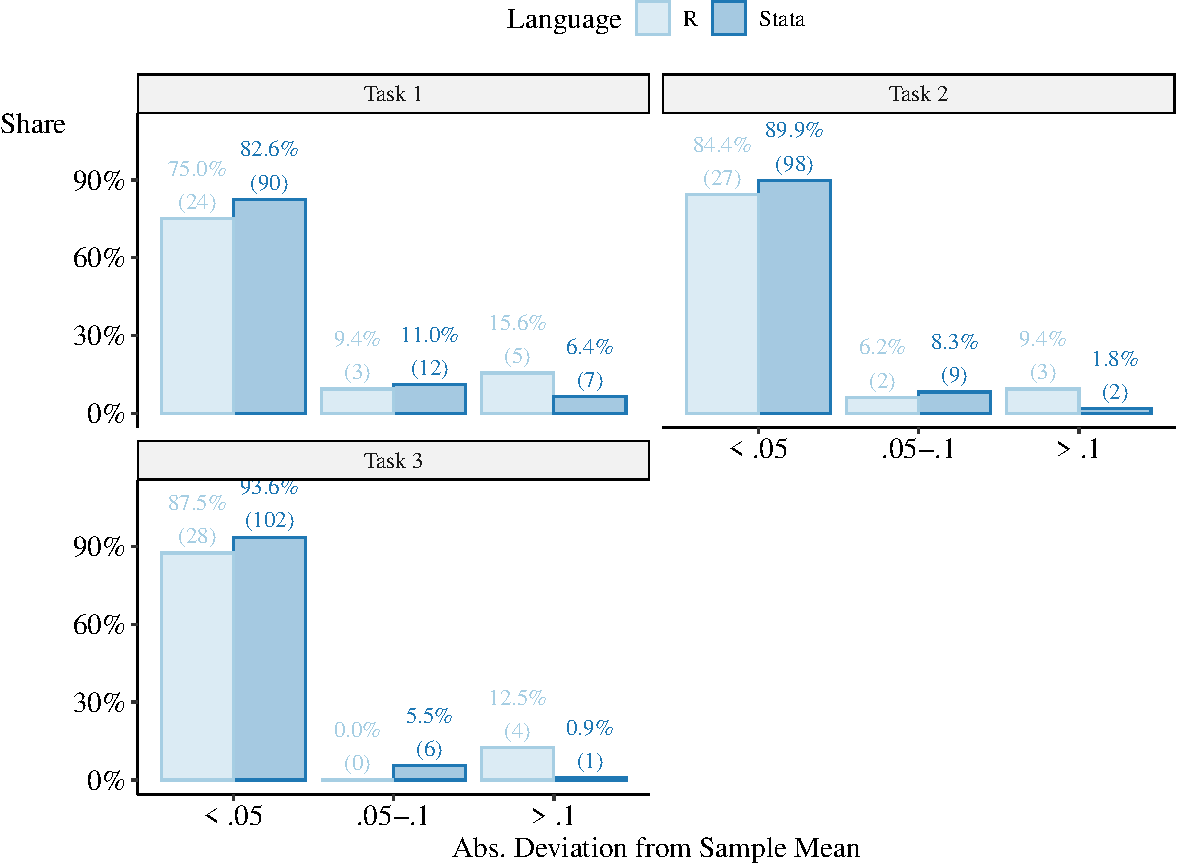
\includegraphics{The-Sources-of-Researcher-Variation-in-Economics_files/figure-pdf/fig-deviations-by-language-1.pdf}

}

\caption{\label{fig-deviations-by-language}Deviation from Sample Mean of
Reported Effect by Language}

\end{figure}

Figure~\ref{fig-deviations-by-language} goes further into the split by
language. We see that, of the two languages, Stata users were more
likely to report effect estimates near the sample mean. 6.4\%, 1.8\%,
and 0.9\% of Stata users were more than .1 in absolute distance from the
sample mean in Tasks 1, 2, and 3, respectively, while for R those values
are 15.6\%, 9.4\%, and 12.5\%. The number of R users is relatively low
at 32,\footnote{This is one lower than the value reported in
  Section~\ref{sec-sample-characteristics} because the researcher who
  was dropped from analysis, mentioned later in
  Section~\ref{sec-sample-characteristics}, was an R user.} and so these
numbers are sensitive to any researchers who were consistently outliers.
There were two R users who had an absolute deviation from the mean of .1
or more every round, while all other R researchers with deviations of .1
or more only had deviations that large in a single round. If we omit
those two consistently-high-deviation R users, the percentages are 10\%,
3.3\%, and 6.7\% for R users, which are still higher than the
percentages for Stata users.

Overall, there is little role for researcher professional or demographic
characteristics in predicting either the level of the effects they
reported, or the deviation of those effects from the mean. There is some
explanatory power for the choice of programming language. R users were
more likely than Stata users to report estimates far from average of
what other users reported.

\hypertarget{analysis-by-project-organizer-b}{%
\subsubsection{Analysis By Project Organizer
B}\label{analysis-by-project-organizer-b}}

Table \ref{tab-researcher-characteristics-regs-b} looks at
within-researcher variation in effect estimates across tasks. In the
first three columns, the dependent variable is the absolute difference
in effects for a given researcher across two tasks, while in the fourth
column, the dependent variable is a researcher's maximum estimated
effect minus their minimum.

\begin{table}
\centering
\caption{Model Coefficients and Standard Errors for Task Comparisons\label{tab-researcher-characteristics-regs-b}}
\centering
\begin{tabular}[t]{lcccc}
\toprule
  & Task 1 vs Task 2 & Task 2 vs Task 3 & Task 1 vs Task 3 & Absolute Range\\
\midrule
Intercept & \num{0.053}*** & \num{0.068}*** & \num{0.053}** & \num{0.087}***\\
 & (\num{0.015}) & (\num{0.018}) & (\num{0.017}) & (\num{0.022})\\
Grad student & \num{0.090}+ & \num{-0.015} & \num{0.099}+ & \num{0.086}\\
 & (\num{0.047}) & (\num{0.054}) & (\num{0.051}) & (\num{0.066})\\
Uni researcher & \num{-0.001} & \num{-0.014} & \num{0.016} & \num{0.000}\\
 & (\num{0.033}) & (\num{0.038}) & (\num{0.036}) & (\num{0.047})\\
Other & \num{0.004} & \num{-0.013} & \num{0.032} & \num{0.011}\\
 & (\num{0.070}) & (\num{0.081}) & (\num{0.077}) & (\num{0.099})\\
Private researcher & \num{0.021} & \num{0.065} & \num{0.134}** & \num{0.110}+\\
 & (\num{0.042}) & (\num{0.049}) & (\num{0.046}) & (\num{0.059})\\
Public researcher & \num{0.047} & \num{-0.013} & \num{0.044} & \num{0.039}\\
 & (\num{0.035}) & (\num{0.041}) & (\num{0.039}) & (\num{0.050})\\
Not PhD & \num{-0.070}+ & \num{0.003} & \num{-0.081}+ & \num{-0.074}\\
 & (\num{0.040}) & (\num{0.047}) & (\num{0.044}) & (\num{0.057})\\
1-5 papers & \num{-0.007} & \num{-0.037} & \num{-0.011} & \num{-0.027}\\
 & (\num{0.021}) & (\num{0.025}) & (\num{0.024}) & (\num{0.030})\\
0 papers & \num{0.012} & \num{-0.047} & \num{-0.017} & \num{-0.026}\\
 & (\num{0.032}) & (\num{0.037}) & (\num{0.035}) & (\num{0.045})\\
\midrule
Num.Obs. & \num{145} & \num{145} & \num{145} & \num{145}\\
R2 & \num{0.046} & \num{0.040} & \num{0.088} & \num{0.047}\\
R2 Adj. & \num{-0.010} & \num{-0.017} & \num{0.034} & \num{-0.009}\\
\bottomrule
\multicolumn{5}{l}{\rule{0pt}{1em}+ p $<$ 0.1, * p $<$ 0.05, ** p $<$ 0.01, *** p $<$ 0.001}\\
\end{tabular}
\end{table}

Most researcher characteristics do not predict absolute
within-researcher variation. Career stage, occupation, and number of
published papers do not predict absolute differences in estimates across
tasks to a statistically significant degree, with few exceptions.

One exception is that private researchers saw larger absolute changes
between Task 1 and Task 3, and also more absolute variation overall,
although the latter is only significant at the \(\alpha = .1\) level.
Probably the most interesting is that inexperience was related to
smaller changes from Task 1 to Task 3: those who do not have a PhD
showed a smaller change between Task 1 and Task 3 (significant at
\(\alpha = .1\)), and those with fewer papers also showed smaller
absolute changes than those with 6+ papers (insignificant).

\hypertarget{two-analyst-results-for-researcher-characteristics}{%
\subsubsection{Two-Analyst Results for Researcher
Characteristics}\label{two-analyst-results-for-researcher-characteristics}}

Both project organizers used the same data to answer the same research
question. From the preregistration: ``Both primary authors will,
independently, analyze the relationship between (a) researcher
characteristics and reported research results in earlier stages, and (b)
attrition from the study and reported research results in later
stages.'' Because there was so little attrition from the study after
Task 1, part b was dropped from the analysis. While this question is
much more open-ended than the main causal inference question in this
paper, it is notable how different the two approaches were. The
dependent variable of interest differed, as did the analytic method and
selection of relevant predictors. Both organizers found, however, that
researcher characterisics were not strong predictors of what the
researchers did.

\hypertarget{sec-bimodal}{%
\subsection{Bimodality in the Task 2 Effect
Estimates}\label{sec-bimodal}}

One of the surprising results in Section~\ref{sec-variation} was the
effect distribution in Task 2. In designing the study, we had expected
that each task would show a narrower distribution of effects than the
previous task. While we did generally see this pattern for sample sizes
and some researcher choices, the distribution of effects in particular
became wider going from Task 1 to Task 2. We also saw some emerging
bimodality, where the larger part of the sample reported estimates that
reflected the distribution of effects already seen in Task 1, while a
smaller group of researchers reported larger effects that were more like
those found in Task 3. In this section we explore possible explanation
for the unexpected findings in Task 2.\footnote{This section is entirely
  un-preregistered, as we did not anticipate this finding.}

The fact that the effect distribution is not just wider but rather
gathers at a high and a low point makes the task of explaining it
somewhat easier, as we can look for features that predict reporting a
higher or lower estimate.

Several anticipated correlates did not explain the bimodal outcomes of
Task 2. Figure~\ref{fig-effect-vs-sample} and
Figure~\ref{fig-effect-vs-se} in the Appendix show that the Task 2
reported sample sizes and standard errors do not strongly explain the
effects reported. Recalling Section~\ref{sec-analytic}, there were not
enormous differences in reported estimates by control variables
included, and there were not covariates associated with large effects
that increased in prominence in Task 2, so it is unlikely that changes
in covariate choice or importance explain the effect distribution.

A possible expanation of the bimodality is that some researchers found
their Task 1 analyses or results ``sticky'' and tried to match them too
closely, while researchers who did not attempt to do this instead
produced results like those in Task 3, since the Task 2 instructions are
very similar to Task 3. However, Figure~\ref{fig-task-1-vs-2} shows
effectively no relationship betwen a given researcher's Task 1 estimate
and their Task 2 estimate.

\begin{figure}

{\centering 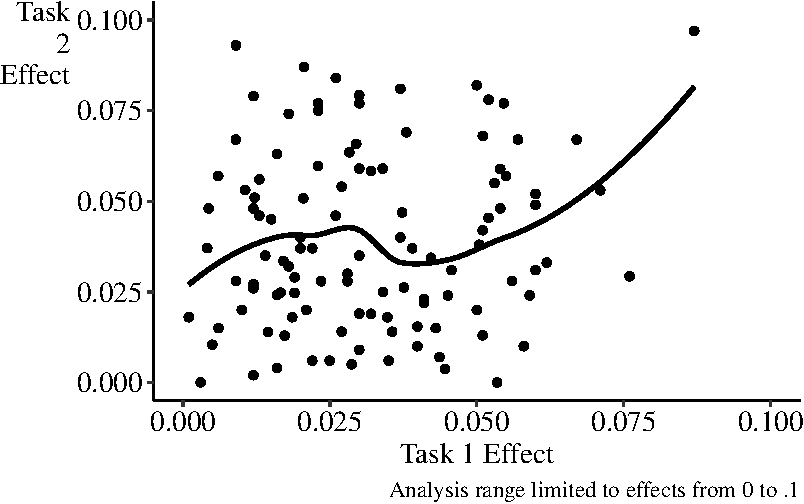
\includegraphics{The-Sources-of-Researcher-Variation-in-Economics_files/figure-pdf/fig-task-1-vs-2-1.pdf}

}

\caption{\label{fig-task-1-vs-2}Estimates Effects in Task 1 vs.~Task 2}

\end{figure}

We then look at sample limitations and definitions. Table
\ref{tab-sample-definition-changes} uses the sample-restriction coding
from Section~\ref{sec-sample-limitations}, and examines whether a given
researcher changed their use of a given variable in their sample
restrictions from Task 1 to Task 2. This could be any change, for
example going from not using the ``Hispanic'' variable at all to using
it, or switching from ``Hispanic-Mexican'' to ``Hispanic-Any''. The
table shows that, with Hispanic and Birthplace as exceptions, the share
above .05 tended to be higher among researchers who changed the way they
used a given variable in defining their sample.

\begin{longtable}[]{@{}
  >{\raggedright\arraybackslash}p{(\columnwidth - 12\tabcolsep) * \real{0.3077}}
  >{\raggedright\arraybackslash}p{(\columnwidth - 12\tabcolsep) * \real{0.1026}}
  >{\raggedleft\arraybackslash}p{(\columnwidth - 12\tabcolsep) * \real{0.0513}}
  >{\raggedright\arraybackslash}p{(\columnwidth - 12\tabcolsep) * \real{0.1154}}
  >{\raggedright\arraybackslash}p{(\columnwidth - 12\tabcolsep) * \real{0.1923}}
  >{\raggedright\arraybackslash}p{(\columnwidth - 12\tabcolsep) * \real{0.1154}}
  >{\raggedright\arraybackslash}p{(\columnwidth - 12\tabcolsep) * \real{0.1154}}@{}}
\caption{Changes in Sample Limitations from Task 1 to 2, and Effect
Changes \label{tab-sample-definition-changes}}\tabularnewline
\toprule\noalign{}
\begin{minipage}[b]{\linewidth}\raggedright
Sample Limitation
\end{minipage} & \begin{minipage}[b]{\linewidth}\raggedright
Changed
\end{minipage} & \begin{minipage}[b]{\linewidth}\raggedleft
N
\end{minipage} & \begin{minipage}[b]{\linewidth}\raggedright
Increase
\end{minipage} & \begin{minipage}[b]{\linewidth}\raggedright
Standard Error
\end{minipage} & \begin{minipage}[b]{\linewidth}\raggedright
R2Effect
\end{minipage} & \begin{minipage}[b]{\linewidth}\raggedright
Abovep05
\end{minipage} \\
\midrule\noalign{}
\endfirsthead
\toprule\noalign{}
\begin{minipage}[b]{\linewidth}\raggedright
Sample Limitation
\end{minipage} & \begin{minipage}[b]{\linewidth}\raggedright
Changed
\end{minipage} & \begin{minipage}[b]{\linewidth}\raggedleft
N
\end{minipage} & \begin{minipage}[b]{\linewidth}\raggedright
Increase
\end{minipage} & \begin{minipage}[b]{\linewidth}\raggedright
Standard Error
\end{minipage} & \begin{minipage}[b]{\linewidth}\raggedright
R2Effect
\end{minipage} & \begin{minipage}[b]{\linewidth}\raggedright
Abovep05
\end{minipage} \\
\midrule\noalign{}
\endhead
\bottomrule\noalign{}
\endlastfoot
Hispanic & No & 110 & -0.01 & 0.01 & 0.04 & 36.4\% \\
Hispanic & Yes & 35 & 0.00 & 0.02 & 0.04 & 22.9\% \\
Birthplace & No & 112 & 0.00 & 0.01 & 0.05 & 35.7\% \\
Birthplace & Yes & 33 & -0.03 & 0.01 & 0.03 & 24.2\% \\
Citizenship & No & 106 & 0.00 & 0.01 & 0.05 & 31.1\% \\
Citizenship & Yes & 39 & -0.02 & 0.02 & 0.04 & 38.5\% \\
Age at Migration & No & 75 & -0.01 & 0.01 & 0.04 & 29.3\% \\
Age at Migration & Yes & 70 & -0.01 & 0.02 & 0.05 & 37.1\% \\
Age in June 2012 & No & 71 & -0.01 & 0.01 & 0.04 & 31.0\% \\
Age in June 2012 & Yes & 74 & -0.01 & 0.02 & 0.05 & 35.1\% \\
Year of Immigration & No & 88 & -0.01 & 0.01 & 0.04 & 28.4\% \\
Year of Immigration & Yes & 57 & 0.00 & 0.02 & 0.05 & 40.4\% \\
Education/Veteran & No & 57 & 0.00 & 0.01 & 0.06 & 31.6\% \\
Education/Veteran & Yes & 88 & -0.02 & 0.02 & 0.03 & 34.1\% \\
Years Continuous in USA & No & 129 & -0.01 & 0.01 & 0.05 & 32.6\% \\
Years Continuous in USA & Yes & 16 & 0.00 & 0.02 & 0.04 & 37.5\% \\
\end{longtable}

Taking the explanatory power of sample restrictions, we then look at the
treated-group definition. Task 2 gave a very precise definition of who
should be included as a part of the treated group. We examine whether a
given researcher followed the full set of treated-group definition
instructions precisely or not. The mismatch could be small, such as
using ``\textless= 16'' instead of ``\textless{} 16'' for age at
migration, or large, such as omitting that eligible people must be
non-citizens. In Figure~\ref{fig-match-vs-mismatch} we show their
distribution of effects against researchers who had a mismatch in their
criteria in any way. The graph shows that the bimodality heavily driven
by the group that precisely matched the treated-group definition. This
implies that the bimodality in Task 2 may be explained in large part by
a split between researchers who exactly followed the instructions, and
so effectively matched what a typical researcher found in Task 3, and
those who did not. This does not fully explain researcher behavior: note
that there is also a weight of researchers with higher results who did
not match perfectly, and also that much of the density of the
perfect-match group is at Task 1 effect levels, but keep in mind that
there are many other decisions in analysis to be made, and this captures
only one angle where determining the correct decision is easiest.

\begin{figure}

{\centering 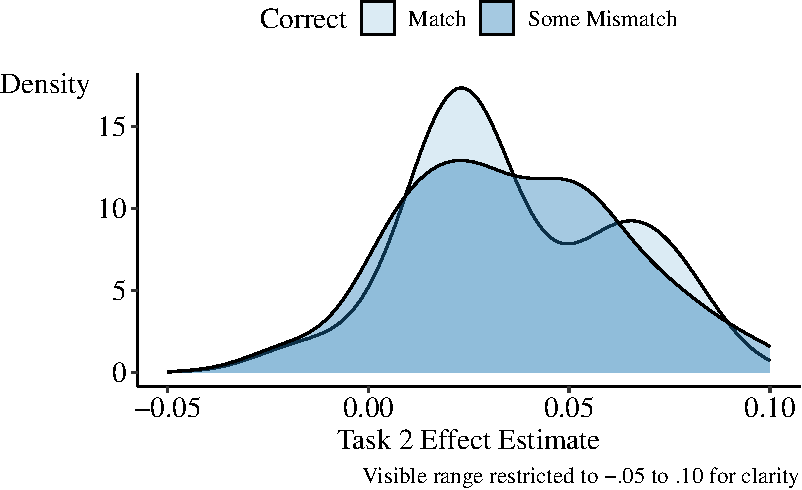
\includegraphics{The-Sources-of-Researcher-Variation-in-Economics_files/figure-pdf/fig-match-vs-mismatch-1.pdf}

}

\caption{\label{fig-match-vs-mismatch}Task 2 Effect Distributions Among
Those with Exact Treated-Group Definition Matchs vs.~Those with Some
Mismatch}

\end{figure}

Further, Table \ref{tab-match-by-field} shows that the share of
researchers matching exactly is fairly low, between 20-25\% by field,
keeping in mind that even very minor mismatches are counted as
mismatches. Further, perfect-match rates were slightly higher among
researchers whose work was closest to the field that the research task
was in, immigration and labor, although this difference was not
statistically significant at the 95\% level.

\begin{longtable}[]{@{}
  >{\raggedright\arraybackslash}p{(\columnwidth - 8\tabcolsep) * \real{0.1867}}
  >{\raggedright\arraybackslash}p{(\columnwidth - 8\tabcolsep) * \real{0.1600}}
  >{\raggedleft\arraybackslash}p{(\columnwidth - 8\tabcolsep) * \real{0.1467}}
  >{\raggedright\arraybackslash}p{(\columnwidth - 8\tabcolsep) * \real{0.2667}}
  >{\raggedleft\arraybackslash}p{(\columnwidth - 8\tabcolsep) * \real{0.2400}}@{}}
\caption{Share of Researchers Matching Treated-Group Definition Exactly
by Field\label{tab-match-by-field}}\tabularnewline
\toprule\noalign{}
\begin{minipage}[b]{\linewidth}\raggedright
Field
\end{minipage} & \begin{minipage}[b]{\linewidth}\raggedright
Share Match
\end{minipage} & \begin{minipage}[b]{\linewidth}\raggedleft
Num. Match
\end{minipage} & \begin{minipage}[b]{\linewidth}\raggedright
Share Some Mismatch
\end{minipage} & \begin{minipage}[b]{\linewidth}\raggedleft
Num Some Mismatch
\end{minipage} \\
\midrule\noalign{}
\endfirsthead
\toprule\noalign{}
\begin{minipage}[b]{\linewidth}\raggedright
Field
\end{minipage} & \begin{minipage}[b]{\linewidth}\raggedright
Share Match
\end{minipage} & \begin{minipage}[b]{\linewidth}\raggedleft
Num. Match
\end{minipage} & \begin{minipage}[b]{\linewidth}\raggedright
Share Some Mismatch
\end{minipage} & \begin{minipage}[b]{\linewidth}\raggedleft
Num Some Mismatch
\end{minipage} \\
\midrule\noalign{}
\endhead
\bottomrule\noalign{}
\endlastfoot
Immigration & 25.0\% & 1 & 75.0\% & 3 \\
Labor & 25.5\% & 12 & 74.5\% & 35 \\
Neither/Other & 22.3\% & 21 & 77.7\% & 73 \\
\end{longtable}

\hypertarget{conclusion}{%
\section{Conclusion}\label{conclusion}}

\hypertarget{recommendations-for-improved-practice}{%
\subsection{Recommendations for Improved
Practice}\label{recommendations-for-improved-practice}}

What do these results imply should change about the practice of applied
microeconomic research?

To some degree, the findings of this paper do not reflect a problem to
be solved. The fact that different researchers approach a problem
differently is not in itself a problem, as long as any points of
disagreement are visible to the reader and subject to scrutiny and
disagreement, and the reader understands that a given study or set of
research decisions is not the last word.

However, there is a problem to be solved to the extent that researcher
variation reflects either (a) error, or (b) choices that are unexamined
or invisible while also being something that researchers would choose
differently.

In this study, we found considerable variation across researchers in the
approaches taken to answering the main question in Task 1, which most
closely reflects actual practice. While the distribution of effects did
not considerably narrow from Task 1 to Task 2, the sample sizes did, as
did the treated and comparison group definitions. Although we generally
did not reject Levene tests of equal variance across rounds,
descriptively there was an obvious narrowing of the distribution of
effects. There was, in both rounds, a lot of variation in the set of
covariates included, as well.

To the extent that these choices reflect research design and modeling
choices, the problem is somewhat already addressed. Researchers are used
to critiquing research design and modeling choices in public work.
Because of this, we would expect that all of these choices would be
reported in a writeup of research, where they could be critiqued. What
would not typically occur is someone actually testing whether many of
these alternate choices actually lead to different results, especially
for seemingly more innocuous choices like covariate functional form,
which was found in this study to be more consequential than the set of
covariates included.

On the part of researcher practice, this set of results suggests the use
of multiverse analysis (Steegen et al. 2016), where the researcher
considers every combination of reasonable modeling decisions and
demonstrates their effects on estimated effects, or even many-analysts
approaches to producing original work, as we did in
Section~\ref{sec-researcher-chars}. On the part of journals, this
suggests that journals should consider accepting work that is a
variation in the approach to a published work, even if that variation is
not framed as a replication or rejection of the original study,
currently a barrier to the publication of replications (Galiani,
Gertler, and Romero 2017).

However, this study did not find that research design and modeling
choices were the majority of explained researcher variation. Instead,
this came in the form of data cleaning and preprocessing, including the
selection of sample and the creation of variables indicating the treated
group. Some of this variation could be classified as error, for example
researchers in Section~\ref{sec-bimodal} whose treated-group definition
in Task 2 did not match the instructions. Other parts of this variation
could be reasonable disagreement.

That much of the relevant variation seems to come along the lines of
data cleaning and preprocessing is possibly unsurprising, given how this
task is currently handled in economics. Relative to modeling and
research design, data cleaning and preprocessing receive little
attention. It is common for minor, or even important, details of data
processing to be left off the description of methods in published
papers. Data cleaning is also not formally taught in most graduate
programs. A professor who would never allow a research assistant to
decide their research design or model might be happy passing along the
data cleaning task to an assistant, even though, as this paper shows,
the task may be just as relevant to the results and just as prone to
arbitrary choice-making.

Because data cleaning gets so little attention, it is perhaps to be
expected that we saw the most variation here. Without formal training in
PhD programs, or a culture of reviewing and critiquing data cleaning and
preprocessing in research papers, there is little opportunity for
researchers to \emph{learn to do the same thing}, and so we see heavy
variation. Contrast this to the popular use of linear probability models
in Table \ref{tab-estimation-methods}, for example, which is common in
applied microeconomics, especially in difference-in-differences designs.
Because its use is very visible, researchers can see that it is the
standard in the field. Whether or not it is actually the best method to
use here, it is a method that researchers know has been agreed upon in
the field. We see a similar story play out with standard error
adjustments in the same table. The standard method by which economists
learn data processing is on a much narrower scale, often from one's
advisor or from others on a small research team.

This problem implies several possible policy solutions. Among broader
system-wide changes, the introduction of data cleaning and preprocessing
classes teaching methods and best practices in the standard PhD applied
economics curriculum would likely improve the quality of economics
research as well as reduce researcher variability. This presumes the
existence of a set of best practices, or at least standard practices.
So, an attempt should be made to codify and popularize a set of
data-cleaning best practices, similar to how applied economists
routinely learn about modeling best practices (for example any number of
econometrics textbooks, or in the applied literature papers like Abadie
et al. (2023)). Other fields have already made strides in this direction
(e.g. Osborne 2012; Jafari 2022) so this effort would not need to start
from scratch, but would be improved by designing recommendations most
relevant to an applied microeconomics context.

Those recommendations may not be in the control of any one researcher,
though. The policy that this paper implies for individual researchers
and journal editors or reviewers is that economics as a field should
consider data cleaning and preprocessing to be just as much a part of
the methods as the choice of model. Researchers should fully describe
their data cleaning processes in their papers to the same level of
detail that they describe their modeling choices. They should also
perhaps subject any arbitrary data-cleaning decisions to multiverse
analysis as well (note that this is also a suggestion of Steegen et al.
(2016)). Further, an increasingly common requirement of journal
submissions is to provide a replication package of the code used to
perform a paper's analyses (for example American Economic Association
(2024)). However, these replication packages often begin from an
already-prepared data set, and only include the code necessary to run
models. It would be advisable to include data preprocessing code in
these replication packages.

\hypertarget{discussion}{%
\subsection{Discussion}\label{discussion}}

This paper describes the results of a large many-analysts project in
applied microeconomics. We found large amounts of variation in the
choices made by researchers, especially in regards to data cleaning and
processing, research design, the definition of treated and comparison
groups, and the selection and functional form of controls. Some of this
variation appears to be from researcher data cleaning processes that do
not match the instructions, derived from policy realities, for
constructing the treated group. Variation was not strongly constrained
by the influence of peer review or a shared research design, but there
was a (descriptive if not statistically significant) reduction of
variation when researchers were provided with pre-cleaned data.

Interestingly, we do not find huge amounts of variation in actual
estimated effects of the policy. There were some outliers, and
statistical significance varied between researchers. However, the
central range of estimated effects of DACA on the probability of working
full time effects generally was not very wide, with the difference
between the 25th and 75th percentiles typically only 2-3 percentage
points. However, the fact that widely different sample definitions and
modeling choices led to a narrow range of effects is not guaranteed to
generalize to other contexts.

There were also parts where researchers behaved very similarly. The use
of linear regression modeling was very popular, and very few researchers
used unadjusted standard errors, although the specific adjustment or
clustering level varied.

What we might learn from this study, and perhaps the wider world of
studies on researcher variation, is perhaps obvious: in cases where
there were well-acknowledged ``standard'' ways of doing something, like
using linear modeling in a difference-in-differences-type setting with a
binary outcome, or adjusting one's standard errors, researchers tended
to do that thing. And where there was no well-acknowledged standard,
like in the choice of clustering level, the selection of covariates in
this particular setting, or in data cleaning, researchers behaved
differently, sometimes to consequence and sometimes without it mattering
much.

While researcher error also plays a part, the impact of the absence of
standards is an emergent result from this study. Readers and
practitioners of research should expect arbitrary variation in parts of
research, like data cleaning, that do not have standards.

The development of best-practice standards in areas where we currently
do not acknowledge them would be likely to improve applied
microeconomics towards being a more mature, sophisticated, and
believable field than it is today. We have highlighted data-cleaning
practices as being an especially fruitful place to develop these
standards, but the same applies in other areas as well like the level of
clustering (an example of a place where development of consensus
guidance is already underway in Abadie et al. (2023)). The optimal level
of researcher variation is not zero, as individual researchers often
have good reasons not to match the methods and practices used by others.
But when this occurs, it should be because there \emph{is} a good reason
to deviate from the template, rather than because we have no template to
begin with.

\hypertarget{references}{%
\section*{References}\label{references}}
\addcontentsline{toc}{section}{References}

\hypertarget{refs}{}
\begin{CSLReferences}{1}{0}
\leavevmode\vadjust pre{\hypertarget{ref-abadie2023should}{}}%
Abadie, Alberto, Susan Athey, Guido W Imbens, and Jeffrey M Wooldridge.
2023. {``When Should You Adjust Standard Errors for Clustering?''}
\emph{The Quarterly Journal of Economics} 138 (1): 1--35.

\leavevmode\vadjust pre{\hypertarget{ref-aeaguidelines}{}}%
American Economic Association. 2024. {``Data and Code Availability
Policy.''} AEA.
\url{https://www.aeaweb.org/journals/data/data-code-policy}.

\leavevmode\vadjust pre{\hypertarget{ref-amuedo2016can}{}}%
Amuedo-Dorantes, Catalina, and Francisca Antman. 2016. {``Can
Authorization Reduce Poverty Among Undocumented Immigrants? Evidence
from the Deferred Action for Childhood Arrivals Program.''}
\emph{Economics Letters} 147: 1--4.

\leavevmode\vadjust pre{\hypertarget{ref-ankel2023economists}{}}%
Ankel-Peters, Jörg, Nathan Fiala, and Florian Neubauer. 2023. {``Do
Economists Replicate?''} \emph{Journal of Economic Behavior \&
Organization} 212: 219--32.

\leavevmode\vadjust pre{\hypertarget{ref-modelsummary2022}{}}%
Arel-Bundock, Vincent. 2022. {``{modelsummary}: Data and Model Summaries
in {R}.''} \emph{Journal of Statistical Software} 103 (1): 1--23.
\url{https://doi.org/10.18637/jss.v103.i01}.

\leavevmode\vadjust pre{\hypertarget{ref-auspurg2021has}{}}%
Auspurg, Katrin, and Josef Brüderl. 2021. {``Has the Credibility of the
Social Sciences Been Credibly Destroyed? Reanalyzing the "Many Analysts,
One Data Set" Project.''} \emph{Socius} 7: 23780231211024421.

\leavevmode\vadjust pre{\hypertarget{ref-auspurg2023social}{}}%
---------. 2023. {``Is Social Research Really Not Better Than Alchemy?
How Many-Analysts Studies Produce {`a Hidden Universe of Uncertainty'}
by Not Following Meta-Analytical Standards.''}

\leavevmode\vadjust pre{\hypertarget{ref-R-data-table}{}}%
Barrett, Tyson, Matt Dowle, Arun Srinivasan, Jan Gorecki, Michael
Chirico, and Toby Hocking. 2024. \emph{Data.table: Extension of
{data.frame}}. \url{https://r-datatable.com}.

\leavevmode\vadjust pre{\hypertarget{ref-bastiaansen2020time}{}}%
Bastiaansen, Jojanneke A, Yoram K Kunkels, Frank J Blaauw, Steven M
Boker, Eva Ceulemans, Meng Chen, Sy-Miin Chow, et al. 2020. {``Time to
Get Personal? The Impact of Researchers Choices on the Selection of
Treatment Targets Using the Experience Sampling Msethodology.''}
\emph{Journal of Psychosomatic Research} 137: 110211.

\leavevmode\vadjust pre{\hypertarget{ref-R-rio}{}}%
Becker, Jason, Chung-hong Chan, David Schoch, and Thomas J. Leeper.
2023. \emph{Rio: A Swiss-Army Knife for Data i/o}.
\url{https://github.com/gesistsa/rio}.

\leavevmode\vadjust pre{\hypertarget{ref-fixest2018}{}}%
Bergé, Laurent. 2018. {``Efficient Estimation of Maximum Likelihood
Models with Multiple Fixed-Effects: The {R} Package {FENmlm}.''}
\emph{CREA Discussion Papers}, no. 13.

\leavevmode\vadjust pre{\hypertarget{ref-boehm2018estimating}{}}%
Boehm, Udo, Jeffrey Annis, Michael J Frank, Guy E Hawkins, Andrew
Heathcote, David Kellen, Angelos-Miltiadis Krypotos, et al. 2018.
{``Estimating Across-Trial Variability Parameters of the Diffusion
Decision Model: Expert Advice and Recommendations.''} \emph{Journal of
Mathematical Psychology} 87: 46--75.

\leavevmode\vadjust pre{\hypertarget{ref-botvinik2020variability}{}}%
Botvinik-Nezer, Rotem, Felix Holzmeister, Colin F Camerer, Anna Dreber,
Juergen Huber, Magnus Johannesson, Michael Kirchler, et al. 2020.
{``Variability in the Analysis of a Single Neuroimaging Dataset by Many
Teams.''} \emph{Nature} 582 (7810): 84--88.

\leavevmode\vadjust pre{\hypertarget{ref-breznau2021observing}{}}%
Breznau, Nate, Eike Mark Rinke, Alexander Wuttke, Muna Adem, Jule
Adriaans, Amalia Alvarez-Benjumea, Henrik Kenneth Andersen, et al. 2021.
{``Observing Many Researchers Using the Same Data and Hypothesis Reveals
a Hidden Universe of Data Analysis.''} \emph{MetaArXiv Preprints}.

\leavevmode\vadjust pre{\hypertarget{ref-broderick2020automatic}{}}%
Broderick, Tamara, Ryan Giordano, and Rachael Meager. 2020. {``An
Automatic Finite-Sample Robustness Metric: When Can Dropping a Little
Data Make a Big Difference?''} \emph{arXiv Preprint arXiv:2011.14999}.

\leavevmode\vadjust pre{\hypertarget{ref-bryan2019replicator}{}}%
Bryan, Christopher J, David S Yeager, and Joseph M O'Brien. 2019.
{``Replicator Degrees of Freedom Allow Publication of Misleading
Failures to Replicate.''} \emph{Proceedings of the National Academy of
Sciences} 116 (51): 25535--45.

\leavevmode\vadjust pre{\hypertarget{ref-callaway2021difference}{}}%
Callaway, Brantly, and Pedro HC Sant'Anna. 2021.
{``Difference-in-Differences with Multiple Time Periods.''}
\emph{Journal of Econometrics} 225 (2): 200--230.

\leavevmode\vadjust pre{\hypertarget{ref-camerer2016evaluating}{}}%
Camerer, Colin F, Anna Dreber, Eskil Forsell, Teck-Hua Ho, Jürgen Huber,
Magnus Johannesson, Michael Kirchler, et al. 2016. {``Evaluating
Replicability of Laboratory Experiments in Economics.''} \emph{Science}
351 (6280): 1433--36.

\leavevmode\vadjust pre{\hypertarget{ref-card2022gender}{}}%
Card, David, Stefano DellaVigna, Patricia Funk, and Nagore Iriberri.
2022. {``Gender Differences in Peer Recognition by Economists.''}
\emph{Econometrica} 90 (5): 1937--71.

\leavevmode\vadjust pre{\hypertarget{ref-chen2024subjectivity}{}}%
Chen, Wanyi, and Mary Cummings. 2024. {``Subjectivity in Unsupervised
Machine Learning Model Selection.''} In \emph{Proceedings of the AAAI
Symposium Series}, 3:22--29. 1.

\leavevmode\vadjust pre{\hypertarget{ref-car2019}{}}%
Fox, John, and Sanford Weisberg. 2019. \emph{An {R} Companion to Applied
Regression}. Third. Thousand Oaks {CA}: Sage.
\url{https://socialsciences.mcmaster.ca/jfox/Books/Companion/}.

\leavevmode\vadjust pre{\hypertarget{ref-galiani2017incentives}{}}%
Galiani, Sebastian, Paul Gertler, and Mauricio Romero. 2017.
{``Incentives for Replication in Economics.''} National Bureau of
Economic Research.

\leavevmode\vadjust pre{\hypertarget{ref-gould2023same}{}}%
Gould, Elliot, Hannah S Fraser, Timothy H Parker, Shinichi Nakagawa,
Simon C Griffith, Peter A Vesk, Fiona Fidler, et al. 2023. {``Same Data,
Different Analysts: Variation in Effect Sizes Due to Analytical
Decisions in Ecology and Evolutionary Biology.''}

\leavevmode\vadjust pre{\hypertarget{ref-herbert2021reproducibility}{}}%
Herbert, Sylvérie, Hautahi Kingi, Flavio Stanchi, and Lars Vilhuber.
2021. {``The Reproducibility of Economics Research: A Case Study.''}

\leavevmode\vadjust pre{\hypertarget{ref-holzmeister2023heterogeneity}{}}%
Holzmeister, Felix, Magnus Johannesson, Robert Böhm, Anna Dreber, Jürgen
Huber, and Michael Kirchler. 2023. {``Heterogeneity in Effect Size
Estimates: Empirical Evidence and Practical Implications.''} Working
Papers in Economics; Statistics.

\leavevmode\vadjust pre{\hypertarget{ref-hoogeveen2023many}{}}%
Hoogeveen, Suzanne, Alexandra Sarafoglou, Balazs Aczel, Yonathan Aditya,
Alexandra J Alayan, Peter J Allen, Sacha Altay, et al. 2023. {``A
Many-Analysts Approach to the Relation Between Religiosity and
Well-Being.''} \emph{Religion, Brain \& Behavior} 13 (3): 237--83.

\leavevmode\vadjust pre{\hypertarget{ref-R-vtable}{}}%
Huntington-Klein, Nick. 2021. \emph{Vtable: Variable Table for Variable
Documentation}. \url{https://nickch-k.github.io/vtable/}.

\leavevmode\vadjust pre{\hypertarget{ref-huntington2021influence}{}}%
Huntington-Klein, Nick, Andreu Arenas, Emily Beam, Marco Bertoni,
Jeffrey R Bloem, Pralhad Burli, Naibin Chen, et al. 2021. {``The
Influence of Hidden Researcher Decisions in Applied Microeconomics.''}
\emph{Economic Inquiry} 59 (3): 944--60.

\leavevmode\vadjust pre{\hypertarget{ref-jafari2022hands}{}}%
Jafari, Roy. 2022. \emph{Hands-on Data Preprocessing in Python: Learn
How to Effectively Prepare Data for Successful Data Analytics}. Packt
Publishing Ltd.

\leavevmode\vadjust pre{\hypertarget{ref-jelveh2024political}{}}%
Jelveh, Zubin, Bruce Kogut, and Suresh Naidu. 2024. {``Political
Language in Economics.''} \emph{The Economic Journal}, ueae026.

\leavevmode\vadjust pre{\hypertarget{ref-klau2023comparing}{}}%
Klau, Simon, Chirag J Patel, John PA Ioannidis, Anne-Laure Boulesteix,
Sabine Hoffmann, et al. 2023. {``Comparing the Vibration of Effects Due
to Model, Data Pre-Processing and Sampling Uncertainty on a Large Data
Set in Personality Psychology.''} \emph{Meta-Psychology} 7.

\leavevmode\vadjust pre{\hypertarget{ref-leamer1983let}{}}%
Leamer, Edward E. 1983. {``Let's Take the Con Out of Econometrics.''}
\emph{The American Economic Review} 73 (1): 31--43.

\leavevmode\vadjust pre{\hypertarget{ref-lundberg2019women}{}}%
Lundberg, Shelly, and Jenna Stearns. 2019. {``Women in Economics:
Stalled Progress.''} \emph{Journal of Economic Perspectives} 33 (1):
3--22.

\leavevmode\vadjust pre{\hypertarget{ref-menkveld2021non}{}}%
Menkveld, Albert J, Anna Dreber, Felix Holzmeister, Juergen Huber,
Magnus Johannesson, Michael Kirchler, Sebastian Neusüss, Michael Razen,
and Utz Weitzel. 2021. {``Non-Standard Errors.''}

\leavevmode\vadjust pre{\hypertarget{ref-open2015estimating}{}}%
Open Science Collaboration. 2015. {``Estimating the Reproducibility of
Psychological Science.''} \emph{Science} 349 (6251): aac4716.

\leavevmode\vadjust pre{\hypertarget{ref-ortloff2023different}{}}%
Ortloff, Anna-Marie, Matthias Fassl, Alexander Ponticello, Florin
Martius, Anne Mertens, Katharina Krombholz, and Matthew Smith. 2023.
{``Different Researchers, Different Results? Analyzing the Influence of
Researcher Experience and Data Type During Qualitative Analysis of an
Interview and Survey Study on Security Advice.''} In \emph{Proceedings
of the 2023 CHI Conference on Human Factors in Computing Systems},
1--21.

\leavevmode\vadjust pre{\hypertarget{ref-osborne2012best}{}}%
Osborne, Jason W. 2012. \emph{Best Practices in Data Cleaning: A
Complete Guide to Everything You Need to Do Before and After Collecting
Your Data}. Sage Publications.

\leavevmode\vadjust pre{\hypertarget{ref-ostropolets2023reproducible}{}}%
Ostropolets, Anna, Yasser Albogami, Mitchell Conover, Juan M Banda,
William A Baumgartner Jr, Clair Blacketer, Priyamvada Desai, et al.
2023. {``Reproducible Variability: Assessing Investigator Discordance
Across 9 Research Teams Attempting to Reproduce the Same Observational
Study.''} \emph{Journal of the American Medical Informatics Association}
30 (5): 859--68.

\leavevmode\vadjust pre{\hypertarget{ref-perignon2022reproducibility}{}}%
Pérignon, Christophe, Olivier Akmansoy, Christophe Hurlin, Anna Dreber,
Felix Holzmeister, Juergen Huber, Michael Kirchler, Michael Razen, et
al. 2022. {``Reproducibility of Empirical Results: Evidence from 1,000
Tests in Finance.''}

\leavevmode\vadjust pre{\hypertarget{ref-portner_huntington-klein_2022}{}}%
Portner, Claus C, and Nick Huntington-Klein. 2022. {``Many
Economists.''} OSF. \url{https://doi.org/10.17605/OSF.IO/CJ9YX}.

\leavevmode\vadjust pre{\hypertarget{ref-ruggles2024ipums}{}}%
Ruggles, Steven, Sarah Flood, Matthew Sobek, Daniel Backman, Annie Chen,
Grace Cooper, Stephanie Richards, Renae Rodgers, and Megan Schouweiler.
2024. {``IPUMS USA: Version 15.0 {[}Dataset{]}. Minneapolis, MN:
IPUMS.''}

\leavevmode\vadjust pre{\hypertarget{ref-sarafoglou2024subjective}{}}%
Sarafoglou, Alexandra, Suzanne Hoogeveen, Don Van Den Bergh, Balázs
Aczél, Casper J Albers, Tim Althoff, Rotem Botvinik-Nezer, et al. 2024.
{``Subjective Evidence Evaluation Survey for Multi-Analyst Studies.''}

\leavevmode\vadjust pre{\hypertarget{ref-schweinsberg2021same}{}}%
Schweinsberg, Martin, Michael Feldman, Nicola Staub, Olmo R van den
Akker, Robbie CM van Aert, Marcel ALM Van Assen, Yang Liu, et al. 2021.
{``Same Data, Different Conclusions: Radical Dispersion in Empirical
Results When Independent Analysts Operationalize and Test the Same
Hypothesis.''} \emph{Organizational Behavior and Human Decision
Processes} 165: 228--49.

\leavevmode\vadjust pre{\hypertarget{ref-silberzahn2018many}{}}%
Silberzahn, Raphael, Eric L Uhlmann, Daniel P Martin, Pasquale Anselmi,
Frederik Aust, Eli Awtrey, Štěpán Bahnı́k, et al. 2018. {``Many Analysts,
One Data Set: Making Transparent How Variations in Analytic Choices
Affect Results.''} \emph{Advances in Methods and Practices in
Psychological Science} 1 (3): 337--56.

\leavevmode\vadjust pre{\hypertarget{ref-simmons2011false}{}}%
Simmons, Joseph P, Leif D Nelson, and Uri Simonsohn. 2011.
{``False-Positive Psychology: Undisclosed Flexibility in Data Collection
and Analysis Allows Presenting Anything as Significant.''}
\emph{Psychological Science} 22 (11): 1359--66.

\leavevmode\vadjust pre{\hypertarget{ref-stansbury2023economics}{}}%
Stansbury, Anna, and Robert Schultz. 2023. {``The Economics Profession's
Socioeconomic Diversity Problem.''} \emph{Journal of Economic
Perspectives} 37 (4): 207--30.

\leavevmode\vadjust pre{\hypertarget{ref-steegen2016increasing}{}}%
Steegen, Sara, Francis Tuerlinckx, Andrew Gelman, and Wolf Vanpaemel.
2016. {``Increasing Transparency Through a Multiverse Analysis.''}
\emph{Perspectives on Psychological Science} 11 (5): 702--12.

\leavevmode\vadjust pre{\hypertarget{ref-sulik2023scientists}{}}%
Sulik, Justin, Nakwon Rim, Elizabeth Pontikes, James Evans, and Gary
Lupyan. 2023. {``Why Do Scientists Disagree?''}

\leavevmode\vadjust pre{\hypertarget{ref-urbaninstdata}{}}%
Urban Institute. 2022. {``State Immigration Policy Resource.''}
\url{https://www.urban.org/data-tools/state-immigration-policy-resource}.

\leavevmode\vadjust pre{\hypertarget{ref-citservices2016}{}}%
U.S. Citizenship and Immigration Services. 2016. {``Number of
i-821D,consideration of Deferred Action for Childhood Arrivals by Fiscal
Year, Quarter, Intake, Biometrics and Case Status: 2012-2016 (June
30).''}

\leavevmode\vadjust pre{\hypertarget{ref-tidyverse2019}{}}%
Wickham, Hadley, Mara Averick, Jennifer Bryan, Winston Chang, Lucy
D'Agostino McGowan, Romain François, Garrett Grolemund, et al. 2019.
{``Welcome to the {tidyverse}.''} \emph{Journal of Open Source Software}
4 (43): 1686. \url{https://doi.org/10.21105/joss.01686}.

\end{CSLReferences}

\FloatBarrier

\appendix

\hypertarget{appendix}{%
\section*{Appendix}\label{appendix}}
\addcontentsline{toc}{section}{Appendix}

\begin{table}
\centering
\caption{Paired Absolute Effect Differences and Peer Review \label{tab-peer-review-reg}}
\centering
\begin{tabular}[t]{lcc}
\toprule
  & Task 1 & Task 2\\
\midrule
Intercept & \num{0.086}*** & \num{0.063}***\\
 & (\num{0.010}) & (\num{0.009})\\
Comparison: Next Round & \num{-0.034}** & \num{-0.006}\\
 & (\num{0.014}) & \vphantom{1} (\num{0.013})\\
Comparison: Next Round vs. This Round & \num{-0.017} & \num{0.000}\\
 & (\num{0.014}) & (\num{0.013})\\
Unreviewed & \num{-0.045}*** & \num{0.001}\\
 & (\num{0.010}) & (\num{0.010})\\
Next Round x Unreviewed & \num{0.057}*** & \num{-0.030}**\\
 & (\num{0.014}) & \vphantom{1} (\num{0.014})\\
Next vs. This x Unreviewed & \num{0.029}** & \num{-0.017}\\
 & (\num{0.014}) & (\num{0.014})\\
\midrule
Num.Obs. & \num{6809} & \num{6676}\\
\bottomrule
\multicolumn{3}{l}{\rule{0pt}{1em}* p $<$ 0.1, ** p $<$ 0.05, *** p $<$ 0.01}\\
\end{tabular}
\end{table}

\begin{figure}

{\centering 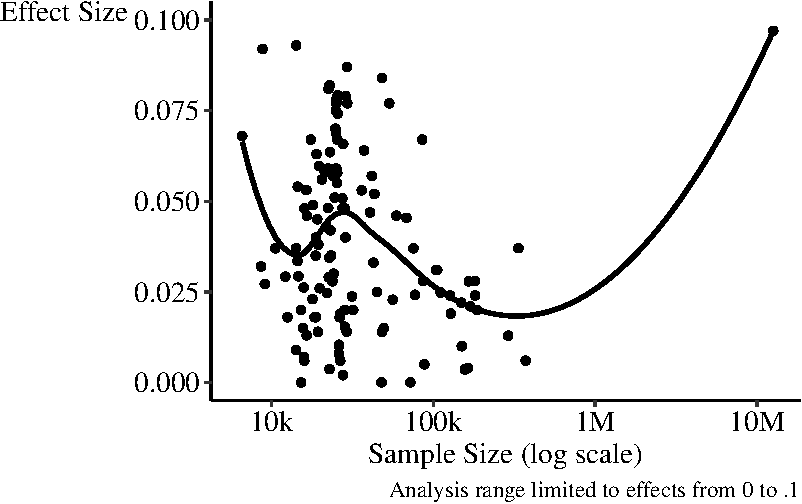
\includegraphics{The-Sources-of-Researcher-Variation-in-Economics_files/figure-pdf/fig-effect-vs-sample-1.pdf}

}

\caption{\label{fig-effect-vs-sample}Task 2 Effect Size and Sample Size}

\end{figure}

\begin{figure}

{\centering 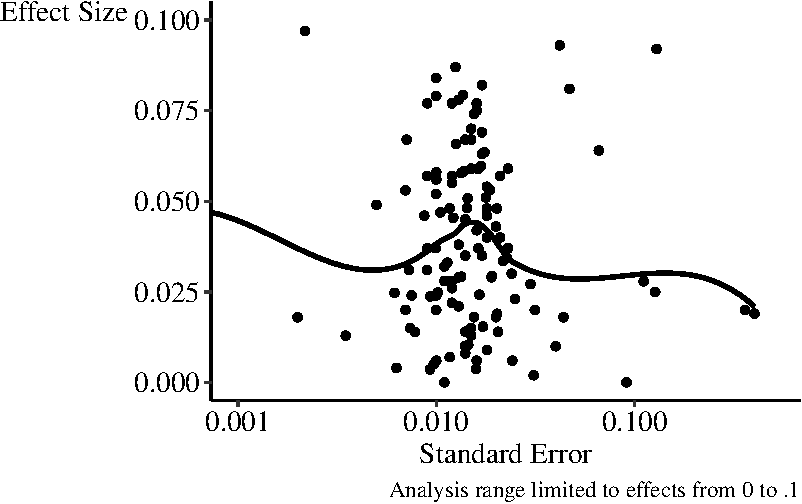
\includegraphics{The-Sources-of-Researcher-Variation-in-Economics_files/figure-pdf/fig-effect-vs-se-1.pdf}

}

\caption{\label{fig-effect-vs-se}Task 2 Effect Size and Standard Error}

\end{figure}

\begin{table}[!htbp] \centering \renewcommand*{\arraystretch}{1.1}\caption{Task 1 Effect and Samples by Sample Definitions, Full View}\label{tab-task1effectsample-full}\resizebox{\textwidth}{!}{
\begin{tabular}{llllllllll}
\hline
\hline
 & \multicolumn{3}{c}{Treated-Group Restriction} & \multicolumn{6}{c}{All-Sample Restriction}  \\ 
 Variable & Effect Pctl. 25 & Pctl. 50 & Pctl. 75 & Effect Pctl. 25 & Pctl. 50 & Pctl. 75 & Samp Size Pctl. 25 & Pctl. 50 & Pctl. 75 \\ 
\hline
Hispanic &  &  &  &  &  &  &  &  &  \\ 
... Hispanic-Mexican & 0.013 & 0.030 & 0.053 & 0.015 & 0.032 & 0.056 & 64,614 & 158,152 & 292,492 \\ 
... Hispanic-Any & 0.030 & 0.037 & 0.050 & 0.030 & 0.045 & 0.054 & 24,276 & 109,759 & 166,270 \\ 
... Hispanic-Mex or Mex-Born & 0.018 & 0.021 & 0.026 & 0.021 & 0.022 & 0.027 & 51,754 & 127,504 & 179,960 \\ 
... Multistep Condition & -0.009 & 0.001 & 0.010 & -0.009 & 0.001 & 0.010 & 326,913 & 366,804 & 406,696 \\ 
... None & 0.015 & 0.023 & 0.052 & 0.012 & 0.022 & 0.048 & 65,124 & 259,630 & 767,657 \\ 
Birthplace &  &  &  &  &  &  &  &  &  \\ 
... Mexican-Born & 0.016 & 0.029 & 0.046 & 0.016 & 0.030 & 0.050 & 61,412 & 141,847 & 276,683 \\ 
... Hispanic-Mex or Mex-Born & 0.041 & 0.100 & 0.160 & 0.004 & 0.016 & 0.070 & 215,436 & 289,311 & 330,348 \\ 
... Non-US Born & -0.020 & -0.020 & -0.020 & -0.013 & -0.007 & -0.001 & 133,992 & 157,710 & 181,428 \\ 
... Central America-Born & 0.057 & 0.057 & 0.057 & 0.057 & 0.057 & 0.057 & 9,711 & 9,711 & 9,711 \\ 
... None & 0.012 & 0.032 & 0.053 & 0.011 & 0.034 & 0.052 & 70,156 & 277,277 & 746,663 \\ 
Citizenship &  &  &  &  &  &  &  &  &  \\ 
... Non-Citizen & 0.017 & 0.030 & 0.051 & 0.022 & 0.035 & 0.056 & 62,920 & 141,847 & 277,270 \\ 
... Foreign-Born & 0.026 & 0.037 & 0.180 & 0.026 & 0.037 & 0.180 & 341,338 & 586,271 & 605,241 \\ 
... Non-Cit or Natlzd post-2012 & 0.001 & 0.022 & 0.028 & 0.017 & 0.017 & 0.017 & 13,377 & 13,377 & 13,377 \\ 
... Citizen (various) & 0.019 & 0.023 & 0.047 & 0.015 & 0.015 & 0.015 & 268,238 & 268,238 & 268,238 \\ 
... Multistep Condition & 0.009 & 0.009 & 0.009 & -0.034 & -0.020 & -0.005 & 899,372 & 1,694,116 & 2,488,861 \\ 
... Other & 0.023 & 0.041 & 0.053 & 0.023 & 0.037 & 0.046 & 13,427 & 17,759 & 84,944 \\ 
... None & 0.010 & 0.021 & 0.051 & 0.010 & 0.020 & 0.043 & 83,476 & 225,894 & 656,161 \\ 
Age at Migration &  &  &  &  &  &  &  &  &  \\ 
... < 16 & 0.016 & 0.030 & 0.050 & 0.018 & 0.026 & 0.046 & 28,348 & 44,288 & 119,180 \\ 
... <= 16 & 0.010 & 0.022 & 0.044 & 0.034 & 0.041 & 0.044 & 120,931 & 204,239 & 205,147 \\ 
... Other & 0.019 & 0.035 & 0.058 & 0.012 & 0.028 & 0.054 & 40,548 & 117,257 & 208,712 \\ 
... None & 0.002 & 0.029 & 0.050 & 0.013 & 0.030 & 0.052 & 95,336 & 255,769 & 507,856 \\ 
Age in June 2012 &  &  &  &  &  &  &  &  &  \\ 
... Year-Quarter Age & 0.015 & 0.030 & 0.052 & 0.017 & 0.029 & 0.051 & 40,661 & 132,637 & 255,734 \\ 
... Year-Only Age & 0.010 & 0.030 & 0.041 & 0.013 & 0.037 & 0.053 & 17,759 & 46,925 & 140,134 \\ 
... None & 0.020 & 0.029 & 0.048 & 0.015 & 0.030 & 0.051 & 90,330 & 206,266 & 424,859 \\ 
Year of Immigration &  &  &  &  &  &  &  &  &  \\ 
... < 2007 & 0.021 & 0.034 & 0.054 & 0.016 & 0.028 & 0.032 & 13,674 & 32,242 & 51,475 \\ 
... <= 2007 & 0.013 & 0.028 & 0.052 & 0.012 & 0.019 & 0.036 & 37,376 & 82,717 & 205,986 \\ 
... < 2012 & 0.014 & 0.014 & 0.014 & 0.039 & 0.051 & 0.064 & 88,982 & 103,534 & 118,086 \\ 
... <= 2012 & 0.042 & 0.118 & 0.194 & 0.029 & 0.092 & 0.155 & 263,220 & 471,364 & 679,507 \\ 
... >= 2007 & 0.012 & 0.012 & 0.012 & 0.012 & 0.012 & 0.012 & 245,635 & 245,635 & 245,635 \\ 
... Any Year & 0.018 & 0.030 & 0.040 & 0.021 & 0.034 & 0.044 & 31,170 & 116,405 & 212,998 \\ 
... Multistep Condition & 0.014 & 0.014 & 0.014 & 0.010 & 0.012 & 0.013 & 137,786 & 170,943 & 204,100 \\ 
... Other & -0.004 & 0.010 & 0.175 & 0.010 & 0.020 & 0.034 & 61,225 & 139,544 & 338,618 \\ 
... None & 0.017 & 0.030 & 0.050 & 0.016 & 0.032 & 0.053 & 110,144 & 230,665 & 474,472 \\ 
Education/Veteran &  &  &  &  &  &  &  &  &  \\ 
... HS Grad or Veteran & 0.043 & 0.065 & 0.088 &  &  &  &  &  &  \\ 
... HS Grad & 0.014 & 0.036 & 0.050 & 0.016 & 0.037 & 0.052 & 66,766 & 132,990 & 169,327 \\ 
... Other & 0.020 & 0.027 & 0.059 & 0.027 & 0.057 & 0.062 & 32,606 & 74,431 & 188,802 \\ 
... None & 0.014 & 0.030 & 0.051 & 0.014 & 0.030 & 0.051 & 62,354 & 203,345 & 387,252 \\ 
Years Continuous in USA &  &  &  &  &  &  &  &  &  \\ 
... Used YRSUSA & 0.017 & 0.030 & 0.052 & 0.019 & 0.026 & 0.045 & 36,523 & 83,097 & 151,054 \\ 
... No YRSUSA & 0.012 & 0.030 & 0.047 & 0.014 & 0.030 & 0.051 & 69,522 & 194,349 & 367,941\\ 
\hline
\hline
\end{tabular}
}
\end{table}

\begin{table}[!htbp] \centering \renewcommand*{\arraystretch}{1.1}\caption{Task 2 Effect and Samples by Sample Definitions, Full View}\label{tab-task2effectsample-full}\resizebox{\textwidth}{!}{
\begin{tabular}{llllllllll}
\hline
\hline
 & \multicolumn{3}{c}{Treated-Group Restriction} & \multicolumn{6}{c}{All-Sample Restriction}  \\ 
 Variable & Effect Pctl. 25 & Pctl. 50 & Pctl. 75 & Effect Pctl. 25 & Pctl. 50 & Pctl. 75 & Samp Size Pctl. 25 & Pctl. 50 & Pctl. 75 \\ 
\hline
Hispanic &  &  &  &  &  &  &  &  &  \\ 
... Hispanic-Mexican & 0.015 & 0.029 & 0.057 & 0.014 & 0.029 & 0.057 & 18,981 & 25,199 & 43,220 \\ 
... Hispanic-Any & 0.028 & 0.050 & 0.063 & 0.024 & 0.042 & 0.058 & 22,983 & 24,011 & 25,568 \\ 
... Hispanic-Mex or Mex-Born & 0.048 & 0.048 & 0.048 &  &  &  &  &  &  \\ 
... Multistep Condition & 0.025 & 0.025 & 0.025 & 0.025 & 0.025 & 0.025 & 44,805 & 44,805 & 44,805 \\ 
... None & 0.020 & 0.040 & 0.067 & 0.023 & 0.043 & 0.075 & 19,106 & 26,396 & 63,634 \\ 
Birthplace &  &  &  &  &  &  &  &  &  \\ 
... Mexican-Born & 0.018 & 0.032 & 0.056 & 0.018 & 0.030 & 0.056 & 19,402 & 25,155 & 38,154 \\ 
... Hispanic-Mex or Mex-Born & 0.070 & 0.070 & 0.070 &  &  &  &  &  &  \\ 
... Non-US Born &  &  &  & 0.028 & 0.045 & 0.058 & 25,498 & 26,138 & 47,180 \\ 
... Central America-Born & 0.067 & 0.067 & 0.067 & 0.067 & 0.067 & 0.067 & 25,538 & 25,538 & 25,538 \\ 
... None & 0.014 & 0.030 & 0.058 & 0.014 & 0.035 & 0.059 & 18,680 & 27,152 & 75,755 \\ 
Citizenship &  &  &  &  &  &  &  &  &  \\ 
... Non-Citizen & 0.018 & 0.031 & 0.058 & 0.019 & 0.033 & 0.058 & 18,834 & 24,979 & 41,917 \\ 
... Foreign-Born &  &  &  & 0.004 & 0.004 & 0.004 & 164,135 & 164,135 & 164,135 \\ 
... Non-Cit or Natlzd post-2012 & 0.014 & 0.034 & 0.048 & 0.019 & 0.024 & 0.029 & 18,162 & 21,823 & 25,484 \\ 
... Citizen (various) & 0.045 & 0.045 & 0.045 & 0.045 & 0.045 & 0.045 & 19,168 & 19,168 & 19,168 \\ 
... Other & 0.020 & 0.049 & 0.059 & 0.031 & 0.059 & 0.059 & 21,828 & 24,011 & 90,368 \\ 
... None & 0.007 & 0.021 & 0.045 & 0.013 & 0.028 & 0.053 & 19,855 & 28,756 & 75,402 \\ 
Age at Migration &  &  &  &  &  &  &  &  &  \\ 
... < 16 & 0.017 & 0.032 & 0.057 & 0.027 & 0.041 & 0.059 & 19,402 & 23,350 & 27,536 \\ 
... <= 16 & 0.008 & 0.021 & 0.045 & 0.014 & 0.020 & 0.038 & 20,392 & 25,199 & 26,267 \\ 
... Other & 0.019 & 0.039 & 0.072 & 0.023 & 0.036 & 0.055 & 16,365 & 24,249 & 49,067 \\ 
... None & 0.023 & 0.037 & 0.065 & 0.013 & 0.026 & 0.053 & 19,367 & 31,458 & 94,773 \\ 
Age in June 2012 &  &  &  &  &  &  &  &  &  \\ 
... Year-Quarter Age & 0.019 & 0.034 & 0.058 & 0.024 & 0.036 & 0.057 & 19,864 & 25,424 & 42,427 \\ 
... Year-Only Age & -0.002 & 0.018 & 0.042 & 0.015 & 0.019 & 0.048 & 16,542 & 26,396 & 29,146 \\ 
... None & 0.008 & 0.018 & 0.049 & 0.007 & 0.026 & 0.059 & 18,803 & 25,414 & 86,316 \\ 
Year of Immigration &  &  &  &  &  &  &  &  &  \\ 
... < 2007 & 0.015 & 0.028 & 0.048 & 0.014 & 0.029 & 0.053 & 22,840 & 25,056 & 28,602 \\ 
... <= 2007 & 0.022 & 0.036 & 0.058 & 0.028 & 0.040 & 0.068 & 20,182 & 25,588 & 28,895 \\ 
... < 2012 & 0.038 & 0.047 & 0.055 &  &  &  &  &  &  \\ 
... <= 2012 & -0.011 & 0.068 & 0.290 & 0.068 & 0.068 & 0.068 & 6,600 & 6,600 & 6,600 \\ 
... >= 2007 & 0.014 & 0.014 & 0.014 &  &  &  &  &  &  \\ 
... Any Year & 0.026 & 0.037 & 0.048 & 0.049 & 0.052 & 0.056 & 18,409 & 20,276 & 22,144 \\ 
... Multistep Condition & 0.000 & 0.017 & 0.035 &  &  &  &  &  &  \\ 
... Other & 0.850 & 0.850 & 0.850 & 0.024 & 0.026 & 0.028 & 25,048 & 35,419 & 45,790 \\ 
... None & 0.013 & 0.035 & 0.057 & 0.013 & 0.028 & 0.056 & 18,803 & 26,127 & 72,235 \\ 
Education/Veteran &  &  &  &  &  &  &  &  &  \\ 
... HS Grad or Veteran & 0.018 & 0.031 & 0.058 & 0.018 & 0.035 & 0.058 & 18,824 & 23,567 & 27,588 \\ 
... 12th Grade or Veteran & 0.049 & 0.067 & 0.091 & 0.061 & 0.067 & 0.073 & 25,473 & 25,532 & 25,590 \\ 
... HS Grad & 0.020 & 0.040 & 0.058 & 0.030 & 0.040 & 0.049 & 18,260 & 21,318 & 24,992 \\ 
... HS Grad or Non-Veteran & 0.026 & 0.047 & 0.051 & 0.023 & 0.037 & 0.052 & 22,687 & 32,814 & 42,521 \\ 
... Other & 0.015 & 0.030 & 0.053 & 0.031 & 0.046 & 0.061 & 18,244 & 24,774 & 43,213 \\ 
... None & 0.005 & 0.018 & 0.059 & 0.007 & 0.026 & 0.052 & 19,802 & 40,272 & 149,084 \\ 
Years Continuous in USA &  &  &  &  &  &  &  &  &  \\ 
... Used YRSUSA & 0.008 & 0.034 & 0.058 & 0.025 & 0.034 & 0.063 & 15,424 & 22,912 & 25,529 \\ 
... No YRSUSA & 0.018 & 0.031 & 0.057 & 0.015 & 0.031 & 0.057 & 19,489 & 25,868 & 52,379\\ 
\hline
\hline
\end{tabular}
}
\end{table}



\end{document}
